\documentclass[11pt,a4paper]{article}
\usepackage[margin=2.3cm]{geometry}
\usepackage[utf8]{inputenc}
\usepackage{amsmath,amssymb,amsthm,mathtools,bm}
\usepackage{xcolor}
\usepackage[most]{tcolorbox}
\usepackage{tikz,pgfplots}
\usetikzlibrary{arrows.meta,calc,positioning,shapes.geometric,fit,backgrounds,decorations.pathreplacing,patterns}
\usepgfplotslibrary{groupplots}
\pgfplotsset{compat=1.17}
\usepackage{booktabs,array,float,enumitem,caption,microtype}
\usepackage[colorlinks=true,linkcolor=blue!50!black,urlcolor=blue!50!black]{hyperref}
\captionsetup{font=small,labelfont=bf}
\setlist{itemsep=2pt,topsep=3pt}
\renewcommand{\thesection}{4.\arabic{section}}

% ---------- macros ----------
\newcommand{\slr}[1]{\texorpdfstring{\emph{(slides~#1)}}{(slides #1)}}
\newcommand{\vx}{\bm{x}}
\newcommand{\vt}{\bm{t}}
\newcommand{\xb}{\bar{\bm{x}}}
\newcommand{\xt}{\tilde{\bm{x}}}
\newcommand{\E}{\bm{E}}
\newcommand{\R}{\bm{R}}
\newcommand{\K}{\bm{K}}
\newcommand{\Rrect}{\bm{R}_{\mathrm{rect}}}
\newcommand{\wL}{\bm{w}_L}
\newcommand{\wR}{\bm{w}_R}
\newcommand{\norm}[1]{\lVert #1\rVert}
\newcommand{\Xhat}{\hat{\bm{X}}}
\DeclareMathOperator*{\argmin}{arg\,min}
\DeclareMathOperator*{\argmax}{arg\,max}
\DeclareMathOperator{\softmax}{softmax}
\DeclareMathOperator{\NN}{NN}
\DeclareMathOperator{\SSD}{SSD}
\DeclareMathOperator{\ZNCC}{ZNCC}

% ---------- boxed amsthm environments ----------
\theoremstyle{definition}
\newtheorem{definition}{Definition}[section]
\newtheorem{lemma}[definition]{Lemma}
\newtheorem{theorem}[definition]{Theorem}
\newtheorem{proposition}[definition]{Proposition}
\newtheorem{corollary}[definition]{Corollary}
\newtheorem{example}[definition]{Example}
\newtheorem{algorithmx}[definition]{Algorithm}

\tcbset{thmbox/.style={enhanced,breakable,boxrule=0.6pt,arc=2pt,left=6pt,right=6pt,top=4pt,bottom=4pt,before skip=8pt,after skip=4pt}}

\newcommand{\newboxedthm}[3]{%
  \NewDocumentEnvironment{#1}{o}{%
    \begin{tcolorbox}[thmbox,colframe=#3!65!black,colback=#3!5]%
    \IfNoValueTF{##1}{\begin{#2}}{\begin{#2}[##1]}}{%
    \end{#2}\end{tcolorbox}}}
\newboxedthm{Definition}{definition}{gray}
\newboxedthm{Lemma}{lemma}{orange}
\newboxedthm{Theorem}{theorem}{red}
\newboxedthm{Proposition}{proposition}{teal}
\newboxedthm{Corollary}{corollary}{purple}
\newboxedthm{Example}{example}{olive}
\newboxedthm{Algorithm}{algorithmx}{brown}

\newtcolorbox{intuition}{enhanced,breakable,colback=blue!5,colframe=blue!60!black,
  fonttitle=\bfseries,title=Intuition,boxrule=0.6pt,arc=2pt,left=6pt,right=6pt,top=3pt,bottom=3pt,
  before skip=4pt,after skip=10pt}

% placeholder for photographs that are not redrawn
\newcommand{\photo}[3]{% #1 slide(s), #2 height, #3 caption
  \begin{figure}[H]\centering
  \begin{tikzpicture}
    \node[draw=gray,dashed,thick,minimum width=0.88\linewidth,minimum height=#2,align=center,text=gray]
      {\textbf{[ INSERT IMAGE ]}\\ take it from slide~#1};
  \end{tikzpicture}
  \caption{#3}
  \end{figure}}

\title{\textbf{Foundations of Spatial AI}\\[2pt] \large 04 -- Stereo Depth Estimation\\[2pt] \normalsize Detailed lecture notes}
\author{Notes based on the slides by L.~Di~Giammarino and E.~Giacomini\\(Sapienza University of Rome)}
\date{October 5, 2026}

\begin{document}
\maketitle

\begin{abstract}\noindent
These notes follow the slide deck \emph{04 Stereo Depth Estimation} (60 slides) section by section; every header carries its slide range. Formal statements (definitions, lemmas, proofs) are merged in where the slides introduce a topic, and blue \emph{Intuition} boxes explain the ``why'' in plain words.
\textbf{Source note:} only the slide deck was uploaded, no companion chapter. The formal content therefore comes from standard references that the slides themselves cite (Hartley--Zisserman / Szeliski for geometry) and from the papers named on the slides (Zbontar--LeCun, Mayer et al., Kendall et al., Wang et al., Leroy et al.). Where a statement goes beyond what the slides say, it is marked as such.
Diagrams are redrawn in TikZ; photographs are left as dashed placeholders that name the slide to copy from.
\end{abstract}

\tableofcontents
\newpage

% =====================================================================
\section*{Agenda and Learning Objectives \slr{1--2}}
\addcontentsline{toc}{section}{Agenda and Learning Objectives (slides 1--2)}
The lecture has five parts: 4.1 Two-View Geometry, 4.2 Block Matching, 4.3 Siamese Networks, 4.4 End-to-End Learning, 4.5 Stereo Without Calibration. After it you should be able to:
\begin{enumerate}
\item explain why calibration and rectification reduce stereo matching to a 1D search, and derive $z=fb/d$ together with its error;
\item explain block matching, its failure modes and the left-right consistency test;
\item describe how learned matching costs and end-to-end networks entered stereo;
\item explain how matching in 3D removes calibration and rectification from the matching step, and what it gives up.
\end{enumerate}

% =====================================================================
\section{Two-View Geometry \slr{3--13}}

\subsection{Depth Cues and Binocular Stereopsis \slr{4}}
Recovering depth from a single image is \emph{ill-posed} (previous lecture). Three ways around it:
\begin{itemize}
\item \textbf{Time-of-flight (ToF)} sensors measure the round-trip time to an obstacle $\Rightarrow$ metric depth.
\item \textbf{Stereo vision} triangulates using two views; because the baseline is known, depth is metric.
\item \textbf{A depth prior} (object assumptions or a neural network) usually gives depth only \emph{up to an affine} transformation.
\end{itemize}
\photo{4}{3.2cm}{Historical and natural binocular systems: Cyclops (cube illusion), stalk-eyed fly, stereoscopic rangefinder (four small photos on the slide).}

\begin{intuition}
Your two eyes are a metric ruler \emph{because} the distance between them is fixed. A single eye (or a monocular network) can say ``this is nearer than that'' but not ``this is 12\,m away''. Stereo trades a second camera for a physical scale.
\end{intuition}

\subsection{Two-View Stereo Matching \slr{5}}
\textbf{Goal:} recover the \emph{disparity} (proportional to inverse depth) for every pixel of a reference image from two input images.
\photo{5}{3.6cm}{Left image, right image and the colour-coded disparity map (Geiger et al., ACCV 2010).}

\subsection{The Classical Stereo Pipeline \slr{6}}
Task: build a dense 3D model of a static scene from two images. Pipeline:
\begin{enumerate}
\item calibrate the cameras intrinsically and extrinsically;
\item rectify the images using the calibration;
\item compute a disparity map for the reference image;
\item remove outliers with a consistency/occlusion test;
\item obtain depth from disparity using the calibration;
\item build a 3D model, e.g.\ by volumetric fusion and meshing.
\end{enumerate}
Steps 1--2 (highlighted on the slide) are exactly what Section~\ref{sec:nocalib} will remove; we revisit this list at the end (\emph{The Pipeline Revisited}).

\subsection{Epipolar Geometry \slr{7}}
\begin{Definition}[Essential matrix]
Let a 3D point $\vx$ project to $\xb_1\propto \K_1\vx$ in camera~1 and to $\xb_2\propto\K_2(\R\vx+\vt)$ in camera~2 ($\xb$ are homogeneous pixel coordinates). The \emph{normalized coordinates} are $\xt_i=\K_i^{-1}\xb_i$. The \emph{essential matrix} is $\E=[\vt]_\times\R$, where $[\vt]_\times$ is the skew-symmetric matrix with $[\vt]_\times\bm v=\vt\times\bm v$.
\end{Definition}

\begin{Proposition}[Epipolar constraint]\label{prop:epi}
Corresponding points satisfy $\xt_2^{\top}\E\,\xt_1=0$. Hence the match of $\xb_1$ lies on the \emph{epipolar line} $\tilde{\bm l}_2=\E\xt_1$ in image~2, and the match of $\xb_2$ lies on $\tilde{\bm l}_1=\E^{\top}\xt_2$ in image~1. All epipolar lines of an image pass through its \emph{epipole}.
\end{Proposition}
\begin{proof}
Up to positive scale, $\xt_1\propto\vx$ and $\xt_2\propto\R\vx+\vt$. Then
$(\R\vx+\vt)^{\top}[\vt]_\times\R\vx=(\R\vx)^{\top}[\vt]_\times(\R\vx)+\vt^{\top}[\vt]_\times\R\vx=0+0,$
because $\bm v^{\top}[\vt]_\times\bm v=0$ and $\vt^{\top}(\vt\times\bm u)=0$ for every $\bm v,\bm u$. Scaling does not change a zero. The statement on lines is the observation that $\xt_2^{\top}\tilde{\bm l}_2=0$ is the equation of a line in image~2.
\end{proof}

\begin{figure}[H]\centering
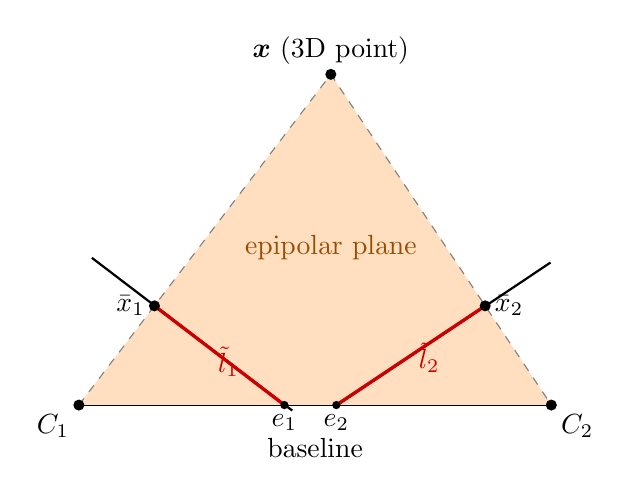
\begin{tikzpicture}[>=Stealth,scale=1.0]
\coordinate (C1) at (0,0); \coordinate (C2) at (6,0); \coordinate (X) at (3.2,4.2);
\coordinate (x1) at (0.96,1.26); \coordinate (x2) at (5.16,1.26);
\coordinate (e1) at (2.61,0); \coordinate (e2) at (3.27,0);
\fill[orange!25] (C1)--(C2)--(X)--cycle;
\draw[thick] (0.165,1.87)--(2.71,-0.07); \draw[thick] (3.25,-0.02)--(5.99,1.81);
\draw[dashed,gray] (C1)--(X)--(C2);
\draw (C1)--(C2);
\draw[red!80!black,very thick] (e1)--(x1); \draw[red!80!black,very thick] (e2)--(x2);
\fill (X) circle (2pt) node[above]{$\bm{x}$ (3D point)};
\fill (C1) circle (2pt) node[below left]{$C_1$}; \fill (C2) circle (2pt) node[below right]{$C_2$};
\fill (x1) circle (2pt) node[left]{$\bar{x}_1$}; \fill (x2) circle (2pt) node[right]{$\bar{x}_2$};
\fill (e1) circle (1.5pt) node[below]{$e_1$}; \fill (e2) circle (1.5pt) node[below]{$e_2$};
\node[red!80!black] at (1.9,0.55) {$\tilde l_1$}; \node[red!80!black] at (4.45,0.6) {$\tilde l_2$};
\node at (3.0,-0.55) {baseline};
\node[orange!60!black] at (3.2,2.0) {epipolar plane};
\end{tikzpicture}
\caption{Epipolar geometry (redrawn from slide~7). The camera centres and the 3D point span the epipolar plane; it cuts each image plane in an epipolar line, and the baseline pierces the image planes at the epipoles.}
\end{figure}

\begin{Example}[Why the 1D search matters]
For a VGA image ($640\times480\approx 307{,}000$ pixels), an unconstrained correspondence search tests about $3\times10^5$ candidates per pixel; searching along one epipolar line tests about $640$. The saving is $480\times$, i.e.\ the image height.
\end{Example}
\begin{intuition}
Given where a pixel sits in image~1, the 3D point can be anywhere along its viewing ray. Seen from camera~2, that ray is a straight line, not a blob: the matching pixel must lie on it. So we ask ``which point \emph{on this line} looks the same?'' instead of ``which point \emph{in the image}?''.
\end{intuition}

\subsection{Image Rectification \slr{8}}
If both cameras face exactly the same direction (image planes co-planar), the epipoles are at infinity and the epipolar lines are parallel: the correspondence of a pixel lies on the \emph{same horizontal scanline}. Real rigs are never perfectly aligned, but we can re-warp both images by a \emph{rotation about the camera centres}, mapping them to a common plane parallel to the baseline; this is \emph{rectification}. Because the rotation is about the camera centre, the 3D structure need not be known.

\begin{figure}[H]\centering
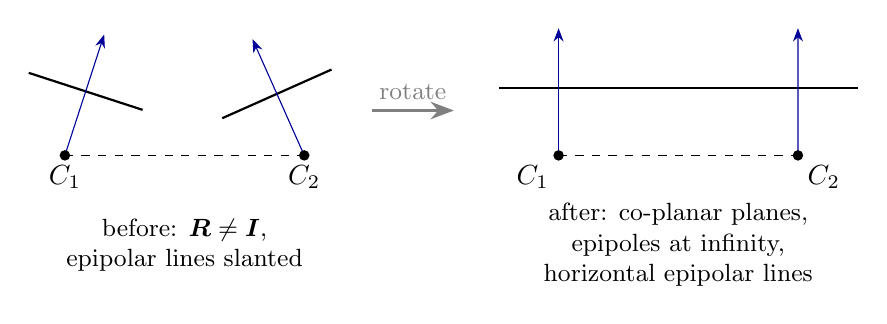
\begin{tikzpicture}[>=Stealth,scale=0.95]
% before
\begin{scope}
\coordinate (A) at (0,0); \coordinate (B) at (3.2,0);
\begin{scope}[shift={(A)},rotate=-18]\draw[thick](-0.8,0.9)--(0.8,0.9);\draw[->,blue!60!black](0,0)--(0,1.7);\end{scope}
\begin{scope}[shift={(B)},rotate=24]\draw[thick](-0.8,0.9)--(0.8,0.9);\draw[->,blue!60!black](0,0)--(0,1.7);\end{scope}
\fill (A) circle(2pt) node[below]{$C_1$}; \fill (B) circle(2pt) node[below]{$C_2$};
\draw[dashed] (A)--(B);
\node[align=center,font=\small] at (1.6,-1.2) {before: $\bm R\neq\bm I$,\\epipolar lines slanted};
\end{scope}
\draw[->,very thick,gray] (4.1,0.6)--(5.2,0.6) node[midway,above]{\small rotate};
\begin{scope}[shift={(6.6,0)}]
\coordinate (A) at (0,0); \coordinate (B) at (3.2,0);
\draw[thick](-0.8,0.9)--(4.0,0.9);
\draw[->,blue!60!black](A)--(0,1.7); \draw[->,blue!60!black](B)--(3.2,1.7);
\fill (A) circle(2pt) node[below left]{$C_1$}; \fill (B) circle(2pt) node[below right]{$C_2$};
\draw[dashed] (A)--(B);
\node[align=center,font=\small] at (1.6,-1.2) {after: co-planar planes,\\epipoles at infinity,\\horizontal epipolar lines};
\end{scope}
\end{tikzpicture}
\caption{Rectification as a pure rotation of each camera (top view; blue arrows are optical axes). After the rotation both image planes are the same plane, parallel to the baseline.}
\end{figure}
\photo{8}{3.4cm}{Example pair of a house before and after rectification, with red horizontal lines (slide 8).}

\subsection{Rectified Epipolar Constraint \slr{9}}
\begin{Proposition}[Rectified setup]\label{prop:rect}
Let $\K_1=\K_2=\R=\bm I$ and $\vt=(t,0,0)^{\top}$. Then
\[
\E=[\vt]_\times=\begin{pmatrix}0&0&0\\0&0&-t\\0&t&0\end{pmatrix},\qquad
\xb_2^{\top}\E\,\xb_1=t\,y_1-t\,y_2=0\ \Longrightarrow\ y_1=y_2 .
\]
\end{Proposition}
\begin{proof}
With $\xb_1=(x_1,y_1,1)^{\top}$ we get $\E\xb_1=(0,-t,t\,y_1)^{\top}$, and $\xb_2^{\top}(0,-t,t\,y_1)^{\top}=-t\,y_2+t\,y_1$. For $t\neq0$ this vanishes iff $y_1=y_2$.
\end{proof}
\begin{intuition}
The only thing separating the two cameras is a sideways slide. A sideways slide moves every point horizontally and never vertically, so the match is on the same row. This is why stereo code can loop along scanlines.
\end{intuition}

\subsection{Calculating the Rectifying Rotation Matrix \slr{10}}
\begin{Lemma}[Rectifying rotation]\label{lem:rectrot}
Let $\R,\vt$ be the relative pose ($\bm x_2=\R\bm x_1+\vt$). Define
\[
\bm r_1=\frac{-\R^{\top}\vt}{\norm{\R^{\top}\vt}_2},\quad
\bm r_2=\frac{[(0,0,1)^{\top}]_\times\bm r_1}{\norm{[(0,0,1)^{\top}]_\times\bm r_1}_2},\quad
\bm r_3=\bm r_1\times\bm r_2,\quad
\Rrect=(\bm r_1,\bm r_2,\bm r_3)^{\top}.
\]
Then $\Rrect$ is a rotation and $\Rrect\bm r_1=(1,0,0)^{\top}$: the epipole of camera~1 becomes an ideal point in the $x$-direction.
\end{Lemma}
\begin{proof}
The centre of camera~2 in the frame of camera~1 solves $\R\bm x+\vt=\bm 0$, i.e.\ $\bm x=-\R^{\top}\vt$; the epipole of image~1 is this direction, so it is $\propto\bm r_1$. By construction $\bm r_2\perp\bm r_1$ (a cross product is orthogonal to its factors), both are unit vectors, and $\bm r_3=\bm r_1\times\bm r_2$ completes a right-handed orthonormal basis. Hence the rows of $\Rrect$ are orthonormal and $\Rrect\bm r_1=(\bm r_1^{\top}\bm r_1,\bm r_2^{\top}\bm r_1,\bm r_3^{\top}\bm r_1)^{\top}=(1,0,0)^{\top}$.
\end{proof}
\begin{Algorithm}[Rectification]
\emph{Input:} two images, intrinsics $\K_1,\K_2$ and relative pose $(\R,\vt)$.\par
\begin{enumerate}[leftmargin=*]
\item Estimate $\E$, decompose it into $\vt$ and $\R$, and build $\Rrect$ as in Lemma~\ref{lem:rectrot}.
\item Warp image~1: $\ \xt_1'=\K\,\Rrect\,\K_1^{-1}\,\xb_1$.
\item Warp image~2: $\ \xt_2'=\K\,\Rrect\,\R^{\top}\,\K_2^{-1}\,\xb_2$.
\end{enumerate}
($\K$ is the common intrinsic matrix of the rectified pair.)
\end{Algorithm}
\begin{intuition}
Think of $\bm r_1$ as ``the direction pointing from camera~1 to camera~2''. Rectification spins both cameras so that this direction becomes the image $x$-axis. Camera~2 first needs undoing its own rotation $\R$ (hence $\R^{\top}$) so that both cameras are spun in the same world frame. The recipe for $\bm r_2$ also explains a limit stated later (slide~34): if the baseline points along the optical axis (forward motion), $\bm r_1\parallel(0,0,1)^{\top}$, the cross product vanishes and $\bm r_2$ is undefined -- planar rectification breaks down.
\end{intuition}

\subsection{Rectified Pair and Disparity \slr{11}}
In a rectified pair the correspondence of a pixel lies in the same image row; the horizontal displacement is the \emph{disparity} $d=x_1-x_2$ (on the slide $0$--$160$\,px, with the match to the left). Disparity is anti-proportional to depth: far points move less than near points.
\photo{11}{4.2cm}{Rectified pair (two lab scenes and a street scene) with colour-coded disparity maps and the 0--160\,px colour bar (slide 11).}

\subsection{Disparity to Depth \slr{12}}
\begin{Theorem}[Triangulation in a rectified pair]\label{thm:depth}
Let the cameras have focal length $f$ (in pixels) and baseline $b$, and let $d=x_1-x_2$ be the disparity of a point at depth $z$. Then
\[ z=\frac{f\,b}{d}. \]
\end{Theorem}
\begin{proof}[Proof (slide version)]
The left and right rays lie in the epipolar plane and intersect at the 3D point; similar triangles give $\frac{z-f}{b-d}=\frac{z}{b}$. Hence $zb-fb=zb-zd$, so $zd=fb$.
\end{proof}
\begin{proof}[Proof (direct)]
Place camera~1 at the origin and camera~2 at $(b,0,0)$. A point $(X,Y,z)$ projects to $x_1=fX/z$ and $x_2=f(X-b)/z$ (principal point at the origin). Subtracting, $d=x_1-x_2=fb/z$.
\end{proof}

\begin{figure}[H]\centering
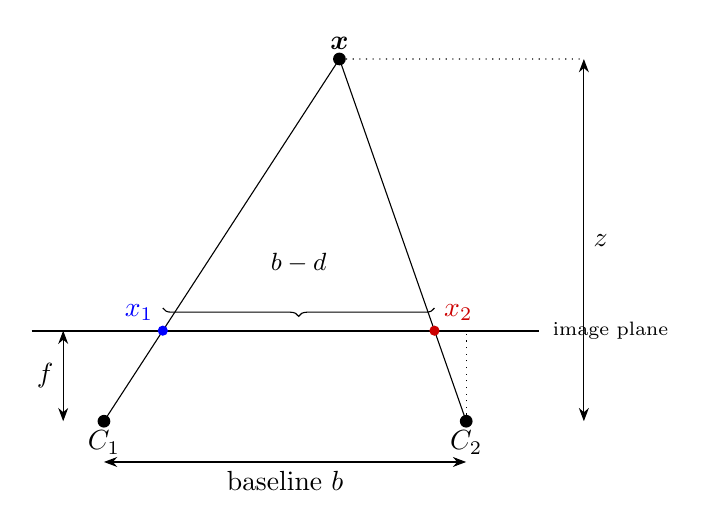
\begin{tikzpicture}[>=Stealth,scale=1.15]
\coordinate (C1) at (0,0); \coordinate (C2) at (4,0); \coordinate (P) at (2.6,4.0);
\draw[thick] (-0.8,1)--(4.8,1) node[left,xshift=-2pt,yshift=8pt,font=\scriptsize]{};
\node[font=\scriptsize,anchor=west] at (4.85,1) {image plane};
\draw (C1)--(P)--(C2);
\fill (P) circle(2pt) node[above]{$\bm{x}$};
\fill (C1) circle(2pt) node[below]{$C_1$}; \fill (C2) circle(2pt) node[below]{$C_2$};
\draw[<->] (0,-0.45)--(4,-0.45) node[midway,below]{baseline $b$};
\draw[<->] (-0.45,0)--(-0.45,1) node[midway,left]{$f$};
\draw[<->] (5.3,0)--(5.3,4) node[midway,right]{$z$};
\draw[dotted] (P)--(5.3,4);
\fill[blue] (0.65,1) circle(1.6pt) node[above left]{$x_1$};
\fill[red!80!black] (3.65,1) circle(1.6pt) node[above right]{$x_2$};
\draw[dotted] (4,0)--(4,1);
\draw[decorate,decoration={brace,amplitude=3pt}] (3.65,1.25)--(0.65,1.25);
\node at (2.15,1.75) {\small $b-d$};
\end{tikzpicture}
\caption{Triangulation (redrawn from slide~12). With $f=1$, $b=4$, $z=4$ in drawing units, each camera measures its own image coordinate ($x_1=0.65$ from $C_1$, $x_2=-0.35$ from $C_2$), so $d=x_1-x_2=1=fb/z$; the similar triangles $(f,\,b-d)$ and $(z,\,b)$ give the formula.}
\end{figure}
\begin{intuition}
Close one eye and point at your thumb, then switch eyes: the thumb jumps a lot. A distant tree barely moves. Disparity \emph{is} that jump, and $z=fb/d$ converts ``how much it jumped'' into ``how far it is''. Doubling the baseline doubles every jump, so a given pixel precision resolves finer depth steps.
\end{intuition}

\subsection{Worked Example: Baseline and Depth Error \slr{13}}
\begin{Theorem}[Depth error]\label{thm:err}
A disparity error $\delta d$ causes, to first order, a depth error
\[ \delta z\approx\left|\frac{\partial z}{\partial d}\right|\delta d=\frac{fb}{d^2}\,\delta d=\frac{z^2}{fb}\,\delta d. \]
\end{Theorem}
\begin{proof}
Differentiate $z=fb\,d^{-1}$: $\partial z/\partial d=-fb/d^2$. Substitute $d=fb/z$ to get $fb/d^2=z^2/(fb)$.
\end{proof}
\begin{Corollary}
The relative error $\delta z/z=z\,\delta d/(fb)$ grows linearly with $z$; doubling $b$ halves $\delta z$ at every depth; if the smallest measurable disparity is $d_{\min}$, the usable range is $z_{\max}=fb/d_{\min}$.
\end{Corollary}
\begin{Example}[Car-like rig, $f\approx721$\,px, $b\approx0.54$\,m, $fb\approx389$\,px$\cdot$m, $\delta d=1$\,px]
\begin{center}\small
\begin{tabular}{@{}ccc@{}}\toprule
depth $z$ & disparity $d$ & depth error $\delta z$\\\midrule
10\,m & 38.9\,px & 0.26\,m\\
20\,m & 19.5\,px & 1.03\,m\\
40\,m & 9.7\,px & 4.11\,m\\\bottomrule
\end{tabular}
\end{center}
(Beyond the slide: the linearisation is first order; with $d-1$ at $z=40$\,m the exact value is $389/8.73-40\approx4.6$\,m.)
\end{Example}
\begin{figure}[H]\centering
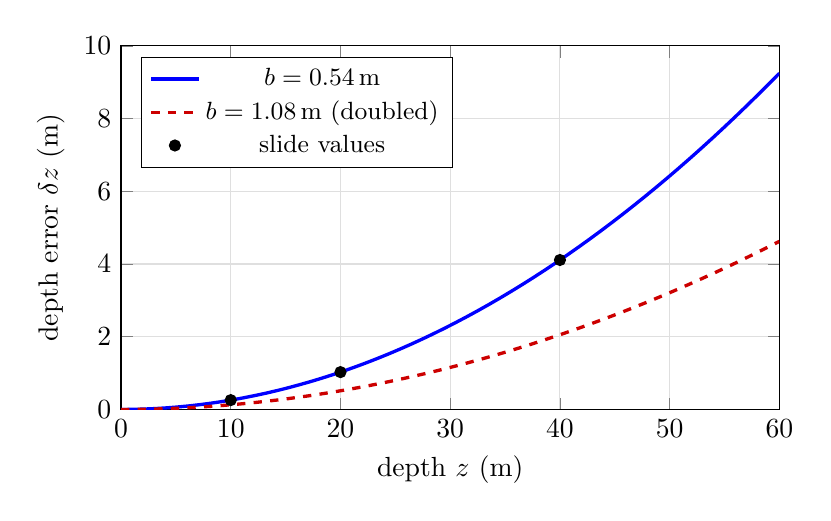
\begin{tikzpicture}
\begin{axis}[width=0.82\linewidth,height=6.2cm,xlabel={depth $z$ (m)},ylabel={depth error $\delta z$ (m)},
 xmin=0,xmax=60,ymin=0,ymax=10,grid=both,grid style={gray!25},legend pos=north west,legend style={font=\small}]
\addplot[blue,very thick,domain=0:60,samples=60]{x^2/389.34};
\addplot[red!80!black,very thick,dashed,domain=0:60,samples=60]{x^2/778.68};
\addplot[only marks,mark=*,mark size=2pt,black] coordinates {(10,0.257)(20,1.027)(40,4.11)};
\legend{$b=0.54$\,m,$b=1.08$\,m (doubled),slide values}
\end{axis}
\end{tikzpicture}
\caption{Depth error for a one-pixel disparity error, $\delta z=z^2\delta d/(fb)$ with $f=721$\,px. The error is quadratic in depth; doubling the baseline halves it everywhere (new figure, not on the slides).}
\end{figure}
\begin{intuition}
At 40\,m the disparity is only 9.7\,px. Being off by one pixel means being off by about 10\,\% of the measurement, and that 10\,\% turns into 4\,m. Near the camera the same one-pixel slip costs a few centimetres. A wider baseline helps the arithmetic, but the two views then differ more and matching gets harder -- the central design tension of stereo.
\end{intuition}

% =====================================================================
\section{Block Matching \slr{14--21}}

\subsection{Correspondence Ambiguity \slr{15}}
How do we decide that two image points correspond? Assume they look ``similar''. But a single pixel does not reveal local structure (ambiguity), so we compare a small patch -- and even then the task is difficult (repetitive or textureless regions, changing appearance).
\photo{15}{3.6cm}{Three grayscale views of an animal with red boxes marking a tail/patch whose appearance changes (slide 15).}

\subsection{Similarity Metrics \slr{16}}
Take two $K\times K$ windows flattened to vectors $\wL,\wR\in\mathbb R^{K^2}$.
\begin{Definition}[SSD and ZNCC]
\begin{align*}
\SSD(x,y,d)&=\norm{\wL(x,y)-\wR(x-d,y)}_2^2,\\
\ZNCC(x,y,d)&=\frac{(\wL-\mu_L)^{\top}(\wR-\mu_R)}{\norm{\wL-\mu_L}_2\,\norm{\wR-\mu_R}_2},
\end{align*}
with $\mu_L,\mu_R$ the means of the two windows (arguments omitted on the right). SSD is a \emph{cost} (minimise); ZNCC is a \emph{similarity} in $[-1,1]$ (maximise).
\end{Definition}
\begin{Lemma}[Gain/bias invariance]\label{lem:zncc}
For $a>0$ and $b\in\mathbb R$, $\ZNCC(a\wL+b\bm 1,\wR)=\ZNCC(\wL,\wR)$. Moreover, for the normalised windows $\hat{\bm w}=(\bm w-\mu)/\norm{\bm w-\mu}_2$ one has $\SSD(\hat{\bm w}_L,\hat{\bm w}_R)=2-2\,\ZNCC(\wL,\wR)$.
\end{Lemma}
\begin{proof}
The mean of $a\wL+b\bm1$ is $a\mu_L+b$, so the centred vector is $a(\wL-\mu_L)$ and its norm $a\norm{\wL-\mu_L}$ (as $a>0$); $a$ cancels in the ratio. For unit vectors $\bm u,\bm v$: $\norm{\bm u-\bm v}^2=2-2\bm u^{\top}\bm v$, and $\hat{\bm w}_L^{\top}\hat{\bm w}_R=\ZNCC$.
\end{proof}
\begin{Example}
Let $\wL=(10,20,30,40)$ and $\wR=\wL+100=(110,120,130,140)$ (same texture, brighter exposure). Then $\SSD=4\cdot100^2=40{,}000$ -- a terrible score -- but $\ZNCC=1$, a perfect match. For the reversed window $(40,30,20,10)$, $\ZNCC=-1$.
\end{Example}
\begin{intuition}
SSD asks ``are the numbers equal?'', ZNCC asks ``do the two patches have the same \emph{pattern of ups and downs}?''. When the two cameras have different gain or exposure, only the second question is the right one. Other metrics exist (Szeliski, Ch.~12.3; Hirschm\"uller and Scharstein, TPAMI 2009).
\end{intuition}

\subsection{Block Matching \slr{17}}
\begin{Algorithm}[Block matching with winner-takes-all]
\emph{Input:} a rectified image pair.\par
\begin{enumerate}[leftmargin=*]
\item Choose a disparity range $[0,d_{\max}]$.
\item For every pixel $(x,y)$ and every $d$, compute the matching cost $C(x,y,d)$ (e.g.\ SSD), giving a \emph{cost volume}.
\item Winner-takes-all: $\hat d(x,y)=\argmin_{d\in[0,d_{\max}]}C(x,y,d)$.
\item Repeat with the roles of the images exchanged and apply the left-right consistency check to remove outliers.
\end{enumerate}
Naively this costs $O(WHD\,K^2)$ per image.
\end{Algorithm}
\begin{figure}[H]\centering
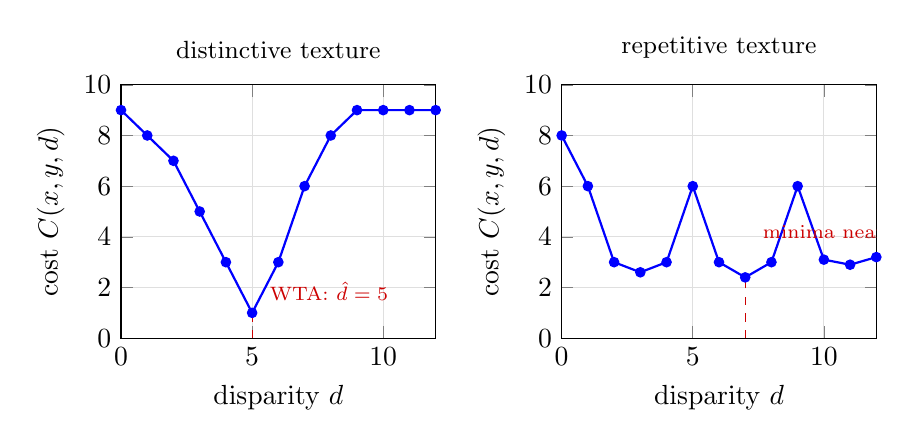
\begin{tikzpicture}
\begin{groupplot}[group style={group size=2 by 1,horizontal sep=1.6cm},width=0.46\linewidth,height=4.8cm,
  xlabel={disparity $d$},ylabel={cost $C(x,y,d)$},ymin=0,ymax=10,xmin=0,xmax=12,grid=both,grid style={gray!25},title style={font=\small}]
\nextgroupplot[title={distinctive texture}]
\addplot[blue,thick,mark=*,mark size=1.5pt] coordinates {(0,9)(1,8)(2,7)(3,5)(4,3)(5,1)(6,3)(7,6)(8,8)(9,9)(10,9)(11,9)(12,9)};
\draw[red!80!black,dashed] (axis cs:5,0)--(axis cs:5,1);
\node[red!80!black,font=\scriptsize,anchor=south west] at (axis cs:5.3,1.1) {WTA: $\hat d=5$};
\nextgroupplot[title={repetitive texture}]
\addplot[blue,thick,mark=*,mark size=1.5pt] coordinates {(0,8)(1,6)(2,3)(3,2.6)(4,3)(5,6)(6,3)(7,2.4)(8,3)(9,6)(10,3.1)(11,2.9)(12,3.2)};
\draw[red!80!black,dashed] (axis cs:7,0)--(axis cs:7,2.4);
\node[red!80!black,font=\scriptsize,anchor=south west] at (axis cs:7.3,3.4) {minima nearly tie};
\end{groupplot}
\end{tikzpicture}
\caption{Illustrative cost curves along one scanline (values invented for illustration, not measured). Left: a clear unique minimum. Right: repeated texture produces several near-equal minima, so noise can make winner-takes-all pick the wrong one.}
\end{figure}
\photo{17}{3.6cm}{Left image, computed disparities (noisy, with holes) and ground truth (slide 17).}
\begin{intuition}
Block matching is a ``find-my-twin'' game on one row: slide a small window of the left image along the row of the right image and keep the position with the lowest cost. Each pixel decides alone -- nobody checks whether neighbours agree -- which is why the output is noisy and why later sections add regularisation and learning.
\end{intuition}

\subsection{Block Matching: Half Occlusions \slr{18}}
A \emph{half-occlusion} is a region visible in the left image but not in the right one (red region on the slide).
\begin{Proposition}[Width of the half-occluded strip]
Let a fronto-parallel foreground with disparity $d_f$ stand in front of a background with disparity $d_b<d_f$. The strip of background that is visible in the left image but hidden in the right image lies immediately left of the foreground's left edge in the left image and has width $d_f-d_b$ pixels.
\end{Proposition}
\begin{proof}
Let the foreground occupy $[a,e]$ in the left image; it appears at $[a-d_f,e-d_f]$ in the right image. A background pixel $x$ of the left image appears at $x-d_b$ in the right image. It is hidden in the right image iff its right-image position $x-d_b$ falls inside the foreground's footprint $[a-d_f,e-d_f]$ while $x<a$ (it is not itself foreground). The condition $x-d_b\ge a-d_f$ reads $x\ge a-(d_f-d_b)$, so the hidden background pixels are exactly $x\in[a-(d_f-d_b),\,a)$, an interval of length $d_f-d_b$.
\end{proof}
\begin{Example}
With the rig of the previous section, a car at 10\,m ($d_f=38.9$\,px) in front of a wall at 40\,m ($d_b=9.7$\,px) hides a strip $29.2$\,px wide next to it. No matching cost can find a twin there, because the twin does not exist.
\end{Example}
\begin{figure}[H]\centering
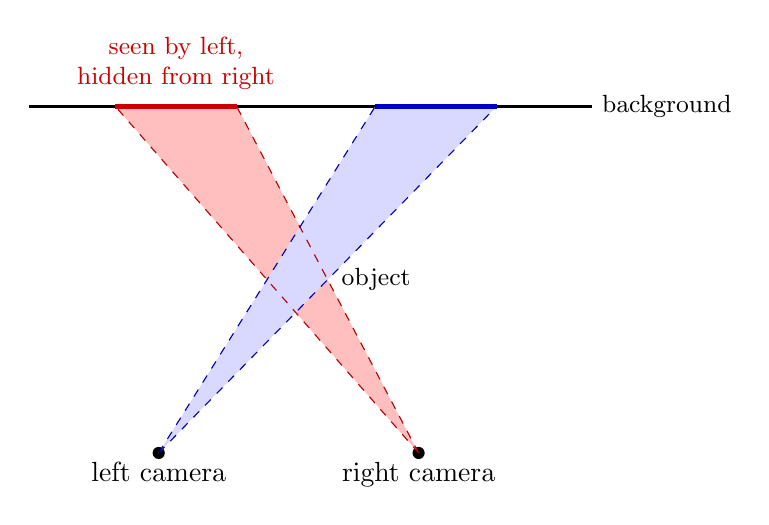
\begin{tikzpicture}[>=Stealth,scale=1.1]
\coordinate (L) at (0,0); \coordinate (R) at (3,0);
\coordinate (P1) at (1.25,2); \coordinate (P2) at (1.95,2);
\draw[thick] (-1.5,4)--(5,4) node[right]{\small background};
\fill[gray] (1.25,1.95) rectangle (1.95,2.05); \node[right] at (2.0,2) {\small object};
\fill (L) circle(2pt) node[below]{left camera}; \fill (R) circle(2pt) node[below]{right camera};
% shadows
\coordinate (rs1) at ($(R)!2!(P1)$); \coordinate (rs2) at ($(R)!2!(P2)$);
\coordinate (ls1) at ($(L)!2!(P1)$); \coordinate (ls2) at ($(L)!2!(P2)$);
\fill[red!25] (R)--(rs1)--(rs2)--cycle;
\fill[blue!15] (L)--(ls1)--(ls2)--cycle;
\draw[red!70!black,dashed] (R)--(rs1); \draw[red!70!black,dashed] (R)--(rs2);
\draw[blue!70!black,dashed] (L)--(ls1); \draw[blue!70!black,dashed] (L)--(ls2);
\draw[red!80!black,ultra thick] (rs1)--(rs2);
\draw[blue!80!black,ultra thick] (ls1)--(ls2);
\node[red!80!black,font=\small,align=center] at (0.2,4.5) {seen by left,\\hidden from right};
\end{tikzpicture}
\caption{Half-occlusion (top view, redrawn from slide~18). Red: background strip hidden from the right camera but visible to the left one; blue: strip hidden from the left camera.}
\end{figure}
\photo{18}{3.3cm}{Left image with the half-occluded region marked in red, zoomed left/right crops, and the occlusion sketch (slide 18).}

\subsection{Block Matching: Assumption Violations \slr{19}}
Block matching assumes that \emph{all pixels inside the window are displaced by the same $d$}: the \emph{fronto-parallel assumption}. It is often wrong: slanted surfaces deform perspectively between views, and at disparity discontinuities the window content changes differently on the two sides.
\begin{Proposition}[Disparity on a plane is affine]
For a plane $\bm n^{\top}\bm X=h$ ($h\neq 0$) in the rectified camera frame, $1/z$ is an affine function of the pixel $(x,y)$; hence so is the disparity $d=fb/z$.
\end{Proposition}
\begin{proof}
A pixel $\xb$ sees $\bm X=z\,\K^{-1}\xb$. Substituting in the plane equation, $z\,\bm n^{\top}\K^{-1}\xb=h$, so $1/z=\bm n^{\top}\K^{-1}\xb/h$, which is linear in $\xb=(x,y,1)^{\top}$. Multiply by $fb$.
\end{proof}
\begin{intuition}
A fronto-parallel wall has constant disparity; a floor or a slanted wall has a disparity that \emph{ramps} across the window. If the ramp is $0.1$\,px per pixel and the window is $11$ pixels wide, the left and right windows disagree by about $1.1$\,px at the edges, enough to hurt the match. Larger windows suffer more.
\end{intuition}
\photo{19}{3.2cm}{Street scene and Teddy-like scene crops showing perspective deformation of windows on slanted surfaces (slide 19).}

\subsection{Effect of Window Size \slr{20}}
\textbf{Trade-off.} Small windows give matching ambiguities and noisy disparity maps. Larger windows give smoother results but lose detail and suffer \emph{border bleeding}: when a window straddles a strong edge, left and right patches get the same disparity because of the dominant edge; the weakly textured background (red on the slide) lacks gradients to overcome it.
\begin{figure}[H]\centering
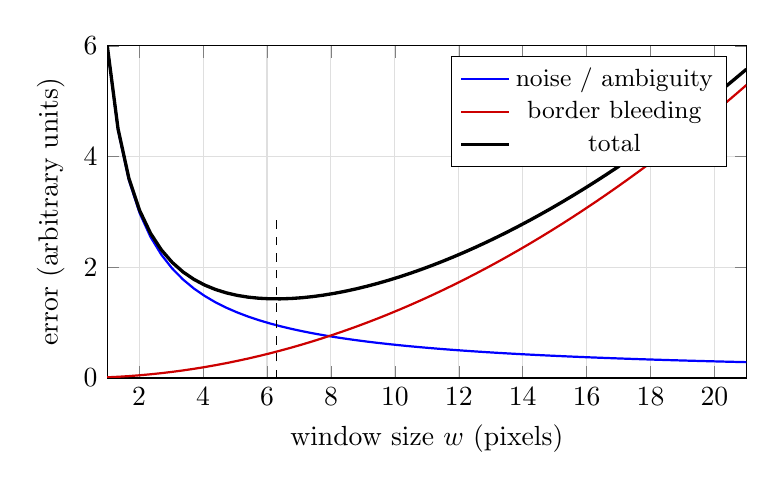
\begin{tikzpicture}
\begin{axis}[width=0.8\linewidth,height=5.8cm,xlabel={window size $w$ (pixels)},ylabel={error (arbitrary units)},
 xmin=1,xmax=21,ymin=0,ymax=6,grid=both,grid style={gray!25},legend pos=north east,legend style={font=\small}]
\addplot[blue,thick,domain=1:21,samples=60]{6/x};
\addplot[red!80!black,thick,domain=1:21,samples=60]{0.012*x^2};
\addplot[black,very thick,domain=1:21,samples=60]{6/x+0.012*x^2};
\legend{noise / ambiguity,border bleeding,total}
\draw[dashed] (axis cs:6.3,0)--(axis cs:6.3,2.9);
\end{axis}
\end{tikzpicture}
\caption{Conceptual bias--variance-style trade-off in window size (illustrative curves, not measured; the slides show it with 5$\times$5 vs 11$\times$11 results).}
\end{figure}
\photo{20}{3.3cm}{Disparity results with 5$\times$5 and 11$\times$11 windows, with ``border bleeding'' regions boxed (slide 20).}

\subsection{Left-Right Consistency Test \slr{21}}
\begin{Definition}[Left-right consistency]
Let $d_L(x,y)$ be the disparity from matching with the left image as reference, and $d_R(x',y)$ the one with the right image as reference. A pixel is \emph{consistent} (kept) if
\[ \bigl|\,d_L(x,y)-d_R\bigl(x-d_L(x,y),\,y\bigr)\bigr|\le\tau, \]
typically with a small threshold $\tau$ (about one pixel); otherwise it is marked invalid. In words: follow the match from left to right and back; you must land where you started (a cycle).
\end{Definition}
\begin{Example}
Left disparities at $x=2,\dots,6$ are $d_L=(2,2,2,4,2)$, so these pixels map to right pixels $x'=x-d_L=(0,1,2,1,4)$. Suppose $d_R(0)=d_R(1)=d_R(2)=d_R(4)=2$. Then the differences $|d_L-d_R(x')|$ are $(0,0,0,2,0)$: with $\tau=1$ the pixel $x=5$ is rejected. Note that $x=3$ and $x=5$ both claim right pixel~1, which is impossible for a surface that is visible in both views.
\end{Example}
\begin{figure}[H]\centering
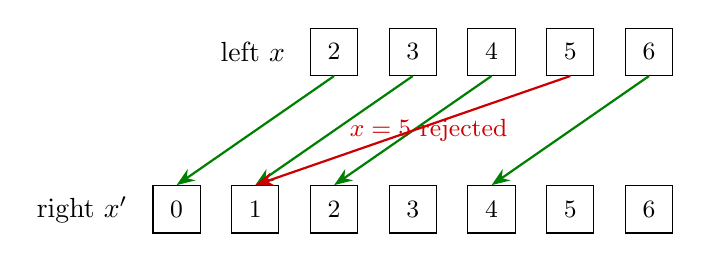
\begin{tikzpicture}[>=Stealth,x=1.0cm,y=1cm]
\foreach \x in {2,...,6}{\node[draw,minimum size=0.6cm,inner sep=0] (L\x) at (\x,2) {\small\x};}
\foreach \x in {0,...,6}{\node[draw,minimum size=0.6cm,inner sep=0] (R\x) at (\x,0) {\small\x};}
\node[left] at (1.5,2) {left $x$}; \node[left] at (-0.5,0) {right $x'$};
\draw[->,green!50!black,thick] (L2.south)--(R0.north);
\draw[->,green!50!black,thick] (L3.south)--(R1.north);
\draw[->,green!50!black,thick] (L4.south)--(R2.north);
\draw[->,red!80!black,thick] (L5.south)--(R1.north);
\draw[->,green!50!black,thick] (L6.south)--(R4.north);
\node[red!80!black,font=\small] at (3.2,1.0) {$x=5$ rejected};
\end{tikzpicture}
\caption{Toy left-to-right matches from the example (new figure). Two left pixels landing on the same right pixel flags an inconsistency.}
\end{figure}
\photo{21}{3.3cm}{Left and right disparity maps used for the consistency check (slide 21).}
\begin{intuition}
Two witnesses must tell the same story: if ``left says my twin is 4 px away'' but ``that twin says its twin is 2 px away'', at least one of them is lying. Half-occluded pixels fail this test automatically, since the supposed twin belongs to something else.
\end{intuition}

% =====================================================================
\section{Siamese Networks \slr{22--28}}
\tikzset{bx/.style={draw,rounded corners=2pt,minimum width=2.5cm,minimum height=0.55cm,font=\scriptsize,fill=blue!6,align=center}}

\subsection{Siamese Networks for Stereo Matching \slr{23}}
Hand-crafted features and similarity metrics do not capture all relevant geometric and radiometric invariances or occlusion patterns; the world is too complex to specify them by hand. Zbontar and LeCun (JMLR 2016) therefore treat \emph{matching cost computation as an image classification problem}:
\begin{itemize}
\item train a CNN patch-wise on image pairs with ground-truth disparity (e.g.\ KITTI Stereo 2015);
\item compute features for each of the two images with the learned model;
\item correlate features between the two images (dot product);
\item take the maximum per pixel (winner-takes-all) or run a global optimisation.
\end{itemize}
\photo{23}{2.8cm}{Small table of left patch / right patch / label (good match, bad match) with traffic-sign crops (slide 23).}

\subsection{Siamese Network Architecture \slr{24}}
Two variants are compared on the slide.
\begin{center}\small
\begin{tabular}{@{}p{0.45\linewidth}p{0.45\linewidth}@{}}\toprule
\textbf{Learned similarity} & \textbf{Cosine similarity}\\\midrule
learn features \emph{and} the similarity metric; potentially more expressive; slow ($W\times H\times D$ MLP evaluations)
& learn features and apply a dot product; the features must do the heavy lifting; fast matching (no network evaluation)\\\bottomrule
\end{tabular}
\end{center}
\begin{figure}[H]\centering
\begin{tikzpicture}[>=Stealth]
% left: learned similarity
\begin{scope}
\node[bx] (a1) at (-1.4,0) {Left patch}; \node[bx] (a2) at (1.4,0) {Right patch};
\node[bx] (b1) at (-1.4,1.0) {Conv+ReLU $\times L$}; \node[bx] (b2) at (1.4,1.0) {Conv+ReLU $\times L$};
\node[bx,minimum width=5.4cm] (c) at (0,2.0) {Concatenate};
\node[bx,minimum width=5.4cm] (d) at (0,3.0) {FC+ReLU $\times2$};
\node[bx,minimum width=5.4cm] (e) at (0,4.0) {FC+Sigmoid};
\node[bx,fill=orange!20,minimum width=5.4cm] (f) at (0,5.0) {similarity score};
\draw[->](a1)--(b1);\draw[->](a2)--(b2);\draw[->](b1)--(-1.4,1.72);\draw[->](b2)--(1.4,1.72);
\draw[->](c)--(d);\draw[->](d)--(e);\draw[->](e)--(f);
\draw[dashed,gray](-0.0,0.7)--(0,1.3) node[midway,right,font=\tiny]{shared};
\node[font=\small\bfseries] at (0,-0.8) {learned similarity};
\end{scope}
% right: cosine
\begin{scope}[shift={(7.2,0)}]
\node[bx] (a1) at (-1.4,0) {Left patch}; \node[bx] (a2) at (1.4,0) {Right patch};
\node[bx] (b1) at (-1.4,1.0) {Conv+ReLU $\times L$}; \node[bx] (b2) at (1.4,1.0) {Conv+ReLU $\times L$};
\node[bx] (n1) at (-1.4,2.0) {Normalize}; \node[bx] (n2) at (1.4,2.0) {Normalize};
\node[bx,minimum width=5.4cm] (c) at (0,3.2) {Dot product};
\node[bx,fill=orange!20,minimum width=5.4cm] (f) at (0,4.2) {similarity score};
\draw[->](a1)--(b1);\draw[->](a2)--(b2);\draw[->](b1)--(n1);\draw[->](b2)--(n2);
\draw[->](n1)--(-1.4,2.9);\draw[->](n2)--(1.4,2.9);\draw[->](c)--(f);
\draw[dashed,gray](0,0.7)--(0,1.3) node[midway,right,font=\tiny]{shared};
\node[font=\small\bfseries] at (0,-0.8) {cosine similarity};
\end{scope}
\end{tikzpicture}
\caption{The two Siamese stereo architectures of Zbontar and LeCun (redrawn from slide~24; layer counts are schematic). Both towers share weights.}
\end{figure}
\begin{Example}[Why the cosine head is fast]
For a KITTI-sized image ($1242\times375$) and $D=228$ candidate disparities, the learned-similarity head needs $WHD\approx1.06\times10^{8}$ network evaluations. The cosine head runs each tower once per image, then each cost is just a dot product of two stored feature vectors.
\end{Example}
\begin{intuition}
Learned similarity is like hiring an expert who inspects every candidate pair. Cosine similarity is like giving every patch a fingerprint once and then comparing fingerprints: much cheaper, but the fingerprint must be good enough that a plain dot product suffices.
\end{intuition}

\subsection{Training Triplets \slr{25}}
\begin{Definition}[Training triplet]
A triplet is $\bigl(\wL(\bm x_L^{\mathrm{ref}}),\ \wR(\bm x_R^{\mathrm{neg}}),\ \wR(\bm x_R^{\mathrm{pos}})\bigr)$ with
\[
\bm x_R^{\mathrm{neg}}=(x_L^{\mathrm{ref}}-d+o_{\mathrm{neg}},\,y_L^{\mathrm{ref}}),\qquad
\bm x_R^{\mathrm{pos}}=(x_L^{\mathrm{ref}}-d+o_{\mathrm{pos}},\,y_L^{\mathrm{ref}}),
\]
where $d$ is the ground-truth disparity, $o_{\mathrm{neg}}\sim\mathcal U(\{-N_{\mathrm{hi}},\dots,-N_{\mathrm{lo}},N_{\mathrm{lo}},\dots,N_{\mathrm{hi}}\})$ and $o_{\mathrm{pos}}\sim\mathcal U(\{-P_{\mathrm{hi}},\dots,P_{\mathrm{hi}}\})$. Typical values: $P_{\mathrm{hi}}=1$, $N_{\mathrm{lo}}=3$, $N_{\mathrm{hi}}=6$.
\end{Definition}
\begin{figure}[H]\centering
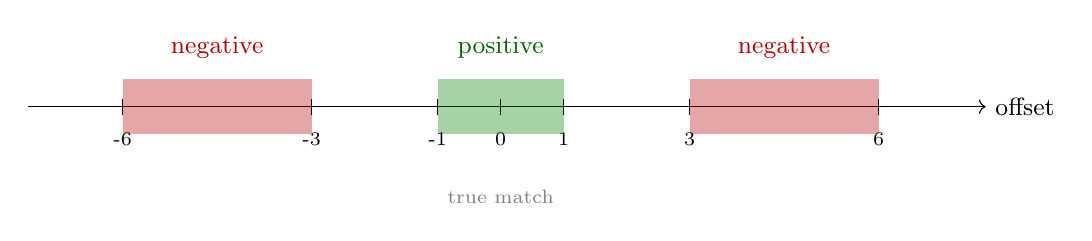
\begin{tikzpicture}[x=0.8cm]
\draw[->] (-7.5,0)--(7.7,0) node[right]{\small offset};
\fill[green!50!black,opacity=0.35] (-1,-0.35) rectangle (1,0.35);
\fill[red!70!black,opacity=0.35] (-6,-0.35) rectangle (-3,0.35);
\fill[red!70!black,opacity=0.35] (3,-0.35) rectangle (6,0.35);
\foreach \x in {-6,-3,-1,0,1,3,6}{\draw (\x,-0.1)--(\x,0.1); \node[below=6pt,font=\scriptsize] at (\x,0) {\x};}
\node[green!40!black,font=\small] at (0,0.75) {positive};
\node[red!70!black,font=\small] at (-4.5,0.75) {negative}; \node[red!70!black,font=\small] at (4.5,0.75) {negative};
\node[font=\scriptsize,gray] at (0,-1.15) {true match};
\end{tikzpicture}
\caption{Where positive and negative right patches are sampled relative to the true match (new figure; ranges $P_{\mathrm{hi}}=1$, $N_{\mathrm{lo}}=3$, $N_{\mathrm{hi}}=6$ from the slide).}
\end{figure}
\photo{25}{3.3cm}{Zoomed right image with a window and rows of green ``positive'' crops and red ``negative'' crops (slide 25).}
\begin{intuition}
Negatives are not random patches: they come from just a few pixels away from the truth ($3$ to $6$\,px), so they look similar and the network must learn the fine cues. Positives are allowed $\pm1$\,px of slack, because a match is never pixel-perfect. Negatives closer than $N_{\mathrm{lo}}$ are excluded since they would be nearly indistinguishable from the positives. This is a mild form of \emph{hard negative mining}. With these values there are $3$ positive and $8$ negative offsets to draw from.
\end{intuition}

\subsection{Hinge Loss \slr{26}}
\begin{Definition}[Hinge (margin) loss]
With $s_+$ and $s_-$ the network scores of the positive and negative example and margin $m>0$,
\[ \mathcal L=\max(0,\,m+s_--s_+). \]
\end{Definition}
\begin{Lemma}
$\mathcal L=0$ iff $s_+\ge s_-+m$. When $\mathcal L>0$, $\partial\mathcal L/\partial s_+=-1$ and $\partial\mathcal L/\partial s_-=+1$: gradient descent raises $s_+$ and lowers $s_-$ at the same rate.
\end{Lemma}
\begin{Example}[$m=0.2$, the value used in the paper]
\begin{center}\small
\begin{tabular}{@{}cccll@{}}\toprule
$s_+$ & $s_-$ & $m+s_--s_+$ & loss & meaning\\\midrule
0.9 & 0.3 & $-0.4$ & 0 & clearly separated, nothing to learn\\
0.6 & 0.5 & $0.1$ & 0.1 & right order but too close: push apart\\
0.4 & 0.7 & $0.5$ & 0.5 & wrong order: large correction\\\bottomrule
\end{tabular}
\end{center}
\end{Example}
\begin{figure}[H]\centering
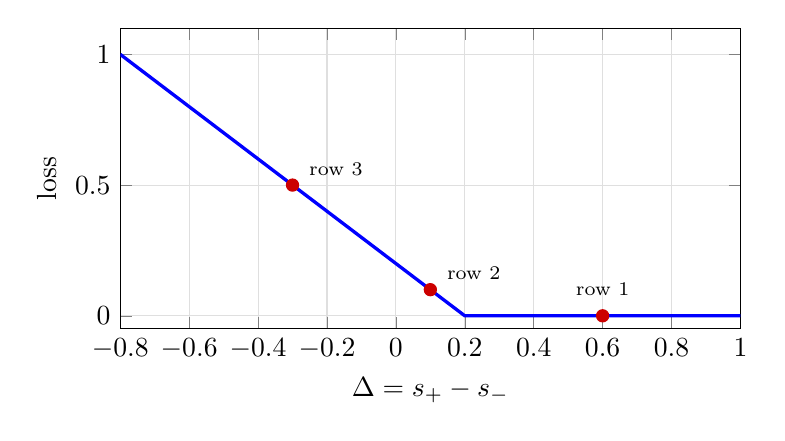
\begin{tikzpicture}
\begin{axis}[width=0.78\linewidth,height=5.4cm,xlabel={$\Delta=s_+-s_-$},ylabel={loss},xmin=-0.8,xmax=1.0,ymin=-0.05,ymax=1.1,grid=both,grid style={gray!25}]
\addplot[blue,very thick,domain=-0.8:1,samples=181]{max(0,0.2-x)};
\addplot[only marks,mark=*,red!80!black,mark size=2.2pt] coordinates {(0.6,0)(0.1,0.1)(-0.3,0.5)};
\node[font=\scriptsize,anchor=south] at (axis cs:0.6,0.04) {row 1};
\node[font=\scriptsize,anchor=south west] at (axis cs:0.12,0.1) {row 2};
\node[font=\scriptsize,anchor=south west] at (axis cs:-0.28,0.5) {row 3};
\end{axis}
\end{tikzpicture}
\caption{Hinge loss with $m=0.2$ as a function of the score gap; red dots are the three rows of the table (new figure).}
\end{figure}
\begin{intuition}
The loss does not demand that the positive scores high in absolute terms, only that it beats the negative by a safety margin. Once it does, the example is ``solved'' and stops contributing -- training focuses its effort on the pairs that are still confusable.
\end{intuition}

\subsection{Comparisons \slr{27}}
The slide compares, on a KITTI street scene, the left input, standard block matching, the Siamese-network matching cost, a semiglobal-matching (SGM, ``optimize'') variant, the left and right disparity maps, and the left-right consistency test. The qualitative message: learned costs are far less noisy than SAD/SSD-style block matching, and adding a global optimisation (SGM) on top improves them further.
\photo{27}{5.0cm}{Grid of six images: left input, Siamese network, standard block matching, left disparity (SGM), right disparity, left-right consistency test (slide 27).}

\subsection{Similarity Constraint: Failure Cases \slr{28}}
The underlying assumption is that \emph{corresponding regions look similar and non-corresponding regions look different}. It fails for: \textbf{repetitions} (several patches look alike), \textbf{textureless surfaces} (everything looks alike), \textbf{occlusions} (the twin does not exist) and \textbf{non-Lambertian surfaces} (the same point looks different from two views, e.g.\ reflections).
The fix suggested on the slide is spatial regularisation (smoothness priors, cf.\ Huang, Lee and Mumford on range-image statistics).
\photo{28}{4.0cm}{Street photo annotated with ``Repetitions'', ``Textureless surfaces'', ``Occlusions'' and ``Non-Lambertian surfaces'' crops (slide 28).}
\begin{intuition}
A matching cost only looks at one pixel (or patch) at a time. When the local evidence is ambiguous or absent, it needs a prior about how the world behaves -- ``neighbouring pixels usually have similar depth'' -- to choose between candidates.
\end{intuition}

% =====================================================================
\section{End-to-End Learning \slr{29--31}}

\subsection{DispNet and Synthetic Data \slr{30}}
\begin{itemize}
\item DispNet (Mayer et al., CVPR 2016) was the first end-to-end trained deep network for stereo.
\item It uses a U-Net-like architecture with skip connections to retain details.
\item A \emph{correlation layer} compares left and right feature maps (the slide notes: 40\,px displacement at feature resolution corresponds to 160\,px in the input image, i.e.\ a stride of 4).
\item Training uses a multi-scale loss (disparity error in pixels) and \emph{curriculum learning} (easy to hard).
\item Pre-train on large \emph{synthetic} datasets (cheap annotations: FlyingThings3D, Monkaa), then fine-tune on a little real data (expensive annotations).
\end{itemize}
\begin{Definition}[1D correlation layer \emph{(general form, not written on the slide)}]
For feature maps $f_L,f_R$ and maximum displacement $D$, a correlation layer outputs the volume $c(x,y,d)=\langle f_L(x,y),f_R(x-d,y)\rangle$ for $d=0,\dots,D$.
\end{Definition}
\begin{figure}[H]\centering
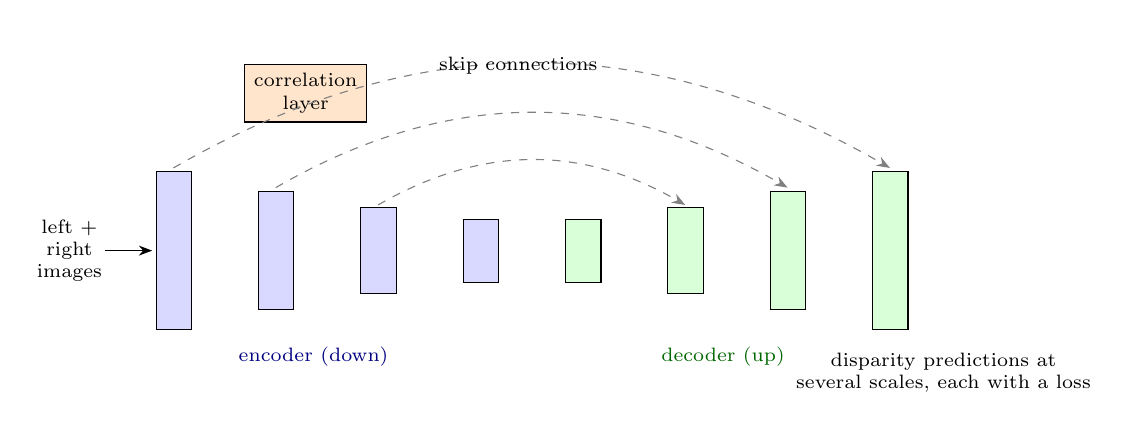
\begin{tikzpicture}[>=Stealth,x=1cm,y=1cm]
\foreach \i/\h in {0/2.0,1/1.5,2/1.1,3/0.8}{\draw[fill=blue!15] (\i*1.3,-\h/2) rectangle (\i*1.3+0.45,\h/2);}
\foreach \i/\h in {4/0.8,5/1.1,6/1.5,7/2.0}{\draw[fill=green!15] (\i*1.3,-\h/2) rectangle (\i*1.3+0.45,\h/2);}
\node[draw,fill=orange!20,font=\scriptsize,align=center] (corr) at (1.9,2.0) {correlation\\layer};
\node[font=\scriptsize,align=center] at (-1.1,0) {left $+$\\right\\images};
\draw[->] (-0.65,0)--(-0.05,0);
\draw[->,dashed,gray] (0.22,1.05) to[bend left=30] (9.32,1.05);
\draw[->,dashed,gray] (1.52,0.8) to[bend left=30] (8.02,0.8);
\draw[->,dashed,gray] (2.82,0.58) to[bend left=30] (6.72,0.58);
\node[font=\scriptsize] at (4.6,2.35) {skip connections};
\node[font=\scriptsize,align=center] at (10.0,-1.55) {disparity predictions at\\several scales, each with a loss};
\node[font=\scriptsize,blue!50!black] at (2.0,-1.35) {encoder (down)}; \node[font=\scriptsize,green!40!black] at (7.2,-1.35) {decoder (up)};
\end{tikzpicture}
\caption{Schematic of a DispNet-style encoder--decoder with skip connections (new schematic, not a reproduction of the slide's network figure).}
\end{figure}
\photo{30}{3.3cm}{DispNet network diagram plus FlyingThings3D and Monkaa sample images (slide 30).}
\begin{intuition}
Hand-designed block matching has no way to ``learn'' that a textureless wall continues smoothly. A network trained on millions of synthetic examples sees every ambiguity, and the U-Net structure lets coarse levels settle the global layout while fine levels sharpen the edges. The synthetic$\to$real recipe exists because perfect ground truth is trivial for a renderer and very costly for real scenes.
\end{intuition}

\subsection{GC-Net \slr{31}}
\textbf{Key idea (Kendall et al., ICCV 2017):} build a \emph{disparity cost volume} and apply \emph{3D convolutions} to it. The learned matching cost $c_\theta(d)$ is converted to a disparity with a differentiable expectation.
\begin{Definition}[Soft argmin]
\[ \hat d=\mathbb E[d]=\sum_{d=0}^{d_{\max}}p(d)\,d,\qquad p(d)=\softmax_d\bigl(-c_\theta(d)\bigr)=\frac{e^{-c_\theta(d)}}{\sum_{k}e^{-c_\theta(k)}}. \]
\end{Definition}
\begin{Proposition}\label{prop:softargmin}
(i) $\hat d\in[0,d_{\max}]$ and $\hat d$ may be non-integer (sub-pixel). (ii) $\hat d$ is differentiable in the costs with
$\dfrac{\partial\hat d}{\partial c(k)}=-p(k)\,\bigl(k-\hat d\bigr).$
\end{Proposition}
\begin{proof}
(i) $p$ is a probability vector, so $\hat d$ is a convex combination of the integers $0,\dots,d_{\max}$. (ii) $\partial p(d)/\partial c(k)=-p(d)(\delta_{dk}-p(k))$, hence
$\partial\hat d/\partial c(k)=\sum_d d\,[-p(d)(\delta_{dk}-p(k))]=-p(k)k+p(k)\hat d$.
\end{proof}
\begin{figure}[H]\centering
\begin{tikzpicture}[>=Stealth]
\tikzset{cube/.style={draw,fill=blue!10}}
\node[bx,minimum width=1.7cm] (img) at (0,0.6) {left\\image}; \node[bx,minimum width=1.7cm] (img2) at (0,-0.6) {right\\image};
\node[bx,minimum width=2.0cm] (c2d) at (2.7,0) {2D conv\\(shared weights)};
\node[bx,minimum width=2.2cm] (cv) at (5.5,0) {cost volume\\$H\times W\times D\times F$};
\node[bx,minimum width=2.2cm] (c3d) at (8.4,0) {3D conv /\\3D deconv};
\node[bx,minimum width=1.8cm] (sa) at (11.0,0) {soft\\argmin};
\node[bx,fill=orange!20,minimum width=1.5cm] (dd) at (13.0,0) {disparity};
\draw[->](img)--(c2d);\draw[->](img2)--(c2d);\draw[->](c2d)--(cv);\draw[->](cv)--(c3d);\draw[->](c3d)--(sa);\draw[->](sa)--(dd);
\end{tikzpicture}
\caption{GC-Net pipeline (redrawn from slide~31).}
\end{figure}
\begin{Example}[Soft argmin on two cost profiles, $d=0,\dots,4$]
\begin{center}\small
\begin{tabular}{@{}lccc@{}}\toprule
 & costs $c(d)$ & $p(d)$ & $\hat d$\\\midrule
unimodal & $(3,1,0,1,3)$ & $(0.027,0.200,0.545,0.200,0.027)$ & $2.0$\\
bimodal & $(0,4,4,4,0)$ & $(0.487,0.009,0.009,0.009,0.487)$ & $2.0$\\\bottomrule
\end{tabular}
\end{center}
\end{Example}
\begin{figure}[H]\centering
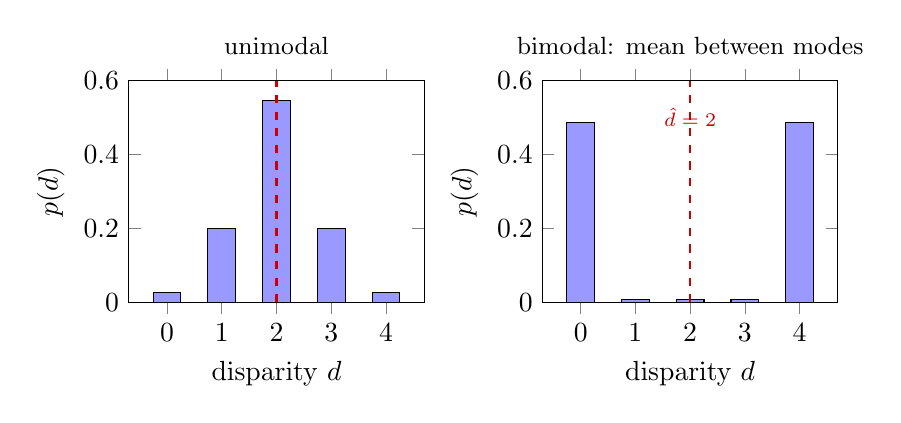
\begin{tikzpicture}
\begin{groupplot}[group style={group size=2 by 1,horizontal sep=1.5cm},width=0.44\linewidth,height=4.4cm,
 xlabel={disparity $d$},ylabel={$p(d)$},ymin=0,ymax=0.6,xtick={0,1,2,3,4},xmin=-0.7,xmax=4.7,title style={font=\small}]
\nextgroupplot[ybar,bar width=10pt,title={unimodal}]
\addplot[fill=blue!40] coordinates {(0,0.027)(1,0.200)(2,0.545)(3,0.200)(4,0.027)};
\draw[red!80!black,thick,dashed] (axis cs:2,0)--(axis cs:2,0.6);
\nextgroupplot[ybar,bar width=10pt,title={bimodal: mean between modes}]
\addplot[fill=blue!40] coordinates {(0,0.487)(1,0.009)(2,0.009)(3,0.009)(4,0.487)};
\draw[red!80!black,thick,dashed] (axis cs:2,0)--(axis cs:2,0.6);
\node[red!80!black,font=\scriptsize,anchor=south] at (axis cs:2,0.45) {$\hat d=2$};
\end{groupplot}
\end{tikzpicture}
\caption{Soft-argmin outputs (red dashed line) for the two profiles of the example. In the bimodal case the expectation is a disparity that neither mode supports (new figure).}
\end{figure}
\begin{Example}[Memory of a 3D volume (illustrative sizes)]
A volume with $H=256$, $W=512$, $D=48$ (disparities at quarter resolution) and $F=32$ float32 channels takes $256\cdot512\cdot48\cdot32\cdot4\approx0.8$\,GB, before any activations of the 3D convolutions are stored for back-propagation.
\end{Example}
\begin{intuition}
An ordinary argmin is a hard decision with no gradient. The soft argmin ``votes'' with weights given by the softmax, which makes the whole network trainable end to end and allows sub-pixel answers. Its weakness is visible in the bimodal row: at an object boundary the cost has two valleys (foreground and background); the expectation averages them and invents a surface in between -- the \emph{smoothness bias} that SMD-Nets later address (backup slides). 3D convolutions add context along the disparity axis at the price of memory (``slightly better performance but large memory requirements'').
\end{intuition}

% =====================================================================
\section{Stereo Without Calibration \slr{32--45}}\label{sec:nocalib}

\subsection{The Cost of Calibration \slr{33}}
Calibration is measured \emph{offline}, with a target, before any image pair is matched. It drifts with temperature, vibration and refocusing; a small rotation error leaves corresponding points on different rows after rectification. Two arbitrary photographs come with no calibration at all and cannot be rectified. The learned stereo networks of Sec.~4.4 inherit all of this: rectified input and a fixed disparity range. (Calibration is the topic of the next lecture.)

\subsection{Limits of Rectification and Local Matching \slr{34}}
\begin{itemize}
\item Forward motion puts the epipole \emph{inside} the image, where planar rectification breaks down (compare the remark after Lemma~\ref{lem:rectrot}).
\item Large rotations between the views distort the rectified images heavily.
\item A wide baseline lowers the depth error (Theorem~\ref{thm:err}) but changes the appearance of every patch, so local matching fails.
\end{itemize}
\photo{34}{4.2cm}{Pair of images with dense colour-coded correspondences under strong camera motion, from MASt3R (slide 34). Caption: ``Dense correspondences where camera motion degrades visual similarity''.}

\subsection{Pointmaps \slr{35}}
\begin{Definition}[Pointmap]
A pointmap $\bm X^{a,1}\in\mathbb R^{H\times W\times3}$ assigns to each pixel $\vx_s$ of image $I_a$, $a\in\{1,2\}$, its 3D point $\bm X^{a,1}[\vx_s]\in\mathbb R^3$ expressed in the frame of camera~1 (the second index names the frame). For image~1 with depth $z$, intrinsics $\K_1$ and augmented pixel $\xb_s$:
\[ \bm X^{1,1}[\vx_s]=z\,\K_1^{-1}\xb_s. \]
\end{Definition}
\emph{DUSt3R} regresses $\Xhat^{1,1}$ and $\Xhat^{2,1}$ from two images -- both in the frame of camera~1 (the hat marks a prediction). Two pixels correspond when their 3D points coincide: \emph{matching becomes a 3D problem}.
\begin{Proposition}[Disparity map as a special case]
For a rectified pair with focal length $f$, principal point $(c_x,c_y)$ and baseline $b$, a pixel $(x,y)$ with disparity $d$ has pointmap entry $\bm X^{1,1}=\dfrac{b}{d}\,(x-c_x,\;y-c_y,\;f)^{\top}$.
\end{Proposition}
\begin{proof}
$z=fb/d$ by Theorem~\ref{thm:depth}, and $\K_1^{-1}\xb=((x-c_x)/f,(y-c_y)/f,1)^{\top}$; multiply.
\end{proof}
\begin{figure}[H]\centering
\begin{tikzpicture}[>=Stealth,scale=1.1]
\coordinate (C1) at (0,0); \coordinate (P) at (2.2,4.2);
\draw[thick] (-1.2,1)--(2.0,1) node[right,font=\scriptsize]{image 1};
\fill (C1) circle(2pt) node[below left]{$C_1$ (origin of the shared frame)};
\draw[->,gray] (C1)--(1,0) node[right,font=\scriptsize]{$X$}; \draw[->,gray] (C1)--(0,0.6) node[above left,font=\scriptsize]{$Y$};
\draw[dashed] (C1)--(P);
\fill[blue] ($(C1)!0.2381!(P)$) circle(1.7pt) node[left,font=\scriptsize]{$\vx_s$};
\fill[red!80!black] (P) circle(2.2pt) node[above right]{$\bm X^{1,1}[\vx_s]=\bm X^{2,1}[\vx_j]$};
\coordinate (C2) at (4.6,0.3);
\fill (C2) circle(2pt) node[below right]{$C_2$};
\draw[dashed] (C2)--(P);
\draw[thick,rotate around={20:(C2)}] ($(C2)+(-1.2,1.0)$)--($(C2)+(1.0,1.0)$);
\node[font=\scriptsize] at (5.6,1.6) {image 2};
\draw[<->] (-1.55,0)--(-1.55,4.2) node[midway,left,font=\scriptsize]{depth $z$};
\end{tikzpicture}
\caption{Pointmaps (new figure). Pixel $\vx_s$ in image~1 and pixel $\vx_j$ in image~2 are \emph{the same 3D point} expressed in camera~1's frame; this is the correspondence criterion.}
\end{figure}
\begin{intuition}
A disparity map stores one number per pixel and only makes sense along a rectified row. A pointmap stores the whole 3D position in a frame shared by both images, so the notion ``these two pixels see the same thing'' becomes simply ``their 3D points are equal'' -- no rows, no calibration of the pair needed to state it.
\end{intuition}

\subsection{The DUSt3R Architecture \slr{36}}
\[ \bm H^a=\mathrm{Encoder}(I_a),\quad \bm H'^1,\bm H'^2=\mathrm{Decoder}(\bm H^1,\bm H^2),\quad \Xhat^{a,1},C^a=\mathrm{Head}_{\mathrm{3D}}\bigl([\bm H^a,\bm H'^a]\bigr). \]
\begin{itemize}
\item \textbf{Siamese encoder:} one ViT-Large (a vision transformer over image patches) encodes both images with \emph{shared weights} into tokens $\bm H^a$.
\item \textbf{Two ViT-Base decoders} exchange information through \emph{cross-attention} and output tokens $\bm H'^a$.
\item \textbf{Heads} regress a pointmap $\Xhat^{a,1}$ and a per-pixel confidence $C^a$ from the concatenated tokens.
\item \textbf{MASt3R} (blue on the slide) extends DUSt3R with local descriptors and fast reciprocal matching.
\end{itemize}
\begin{figure}[H]\centering
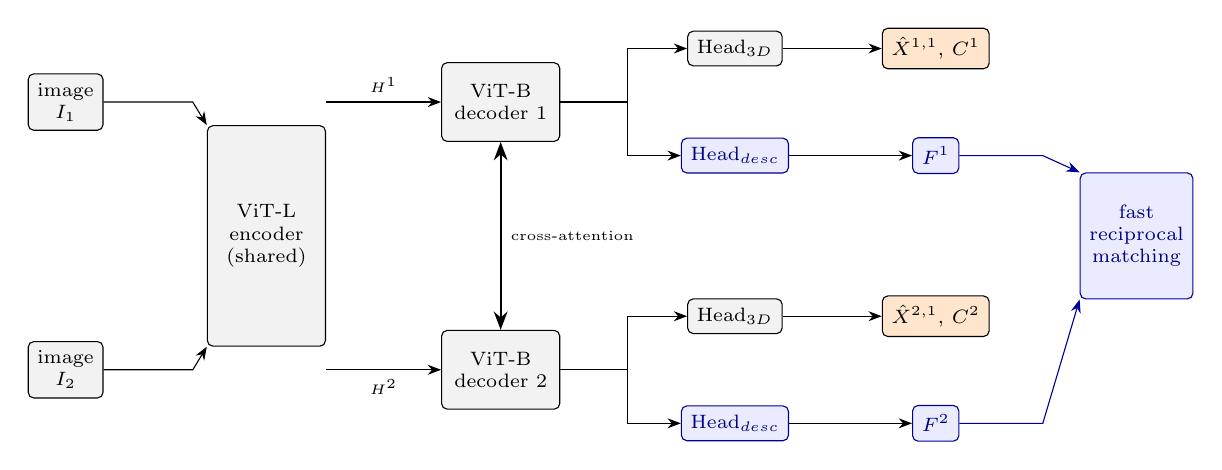
\begin{tikzpicture}[>=Stealth,x=0.85cm,y=0.85cm]
\tikzset{nb/.style={draw,rounded corners=2pt,font=\scriptsize,align=center,fill=gray!10},nbb/.style={draw=blue!60!black,text=blue!50!black,rounded corners=2pt,font=\scriptsize,align=center,fill=blue!8}}
\node[nb] (i1) at (0,2) {image\\$I_1$}; \node[nb] (i2) at (0,-2) {image\\$I_2$};
\node[nb,minimum height=2.8cm,minimum width=1.5cm] (enc) at (3,0) {ViT-L\\encoder\\(shared)};
\node[nb,minimum width=1.5cm,minimum height=1.0cm] (d1) at (6.5,2) {ViT-B\\decoder 1}; \node[nb,minimum width=1.5cm,minimum height=1.0cm] (d2) at (6.5,-2) {ViT-B\\decoder 2};
\node[nb] (h3a) at (10,2.8) {Head$_{3D}$}; \node[nbb] (hda) at (10,1.2) {Head$_{desc}$};
\node[nb] (h3b) at (10,-1.2) {Head$_{3D}$}; \node[nbb] (hdb) at (10,-2.8) {Head$_{desc}$};
\node[nb,fill=orange!20] (o3a) at (13,2.8) {$\hat X^{1,1},\,C^1$}; \node[nbb] (oda) at (13,1.2) {$F^1$};
\node[nb,fill=orange!20] (o3b) at (13,-1.2) {$\hat X^{2,1},\,C^2$}; \node[nbb] (odb) at (13,-2.8) {$F^2$};
\node[nbb,minimum height=1.6cm] (nn) at (16,0) {fast\\reciprocal\\matching};
\draw[->](i1.east)--(1.9,2)--(enc.north west);
\draw[->](i2.east)--(1.9,-2)--(enc.south west);
\draw[->](enc.east|-d1)--(d1) node[midway,above,font=\tiny]{$H^1$}; \draw[->](enc.east|-d2)--(d2) node[midway,below,font=\tiny]{$H^2$};
\draw[<->,thick](d1.south)--(d2.north) node[midway,right,font=\tiny]{cross-attention};
\draw[->](d1.east)--(8.4,2)--(8.4,2.8)--(h3a.west); \draw[->](8.4,2)--(8.4,1.2)--(hda.west);
\draw[->](d2.east)--(8.4,-2)--(8.4,-1.2)--(h3b.west); \draw[->](8.4,-2)--(8.4,-2.8)--(hdb.west);
\draw[->](h3a)--(o3a);\draw[->](hda)--(oda);\draw[->](h3b)--(o3b);\draw[->](hdb)--(odb);
\draw[->,blue!60!black](oda.east)--(14.6,1.2)--(nn.north west); \draw[->,blue!60!black](odb.east)--(14.6,-2.8)--(nn.south west);
\end{tikzpicture}
\caption{DUSt3R/MASt3R architecture (redrawn from slides~36 and~39; blue = MASt3R additions).}
\end{figure}
\photo{36}{3.2cm}{Photos at the left (input images) and right (resulting geometric matching and feature-based fast matching visuals) of the architecture figure (slide 36).}
\begin{intuition}
The encoder turns each image into a bag of patch tokens independently; the decoders then let the two images ``talk'' through cross-attention so that each token can relate to the other view. The heads translate tokens into per-pixel 3D coordinates. Crucially, both outputs are in the \emph{same} frame, which is what makes 3D matching possible.
\end{intuition}

\subsection{MASt3R Network Output \slr{37}}
Per image, the network outputs three dense maps: a pointmap $\Xhat\in\mathbb R^{H\times W\times3}$ (with $\Xhat[i]\in\mathbb R^3$), a confidence $C\in\mathbb R^{H\times W}$ (with $C[i]\in\mathbb R$) and a local descriptor map $F\in\mathbb R^{H\times W\times24}$ (with $F[i]\in\mathbb R^{24}$).
\photo{37}{3.0cm}{Three 3D-slab sketches: pointmap $\hat X$, confidence $C$ and local feature $F$ with a highlighted pixel (slide 37).}

\subsection{Training Objective and Metric Scale \slr{38}}
\begin{Definition}[Confidence-weighted regression loss]
With $\rho,\hat\rho$ the mean distances of the valid ground-truth and predicted points to the origin,
\[
\ell_{\mathrm{regr}}(a,i)=\Bigl\lVert\tfrac1{\hat\rho}\Xhat^{a,1}[i]-\tfrac1\rho\bm X^{a,1}[i]\Bigr\rVert,\qquad
\mathcal L_{\mathrm{conf}}=\sum_{a\in\{1,2\}}\sum_{i\in\mathcal V^a}C^a[i]\,\ell_{\mathrm{regr}}(a,i)-\alpha\log C^a[i],
\]
$\mathcal V^a$ the pixels of $I_a$ with valid ground truth, $\alpha=0.2$. Dividing by $\rho,\hat\rho$ removes the unknown scale.
\end{Definition}
\begin{Proposition}[Optimal confidence]
For a fixed error $\ell>0$, the function $C\mapsto C\ell-\alpha\log C$ on $C>0$ is minimised at $C^\ast=\alpha/\ell$, with minimum value $\alpha\bigl(1+\log(\ell/\alpha)\bigr)$.
\end{Proposition}
\begin{proof}
The derivative $\ell-\alpha/C$ vanishes at $C=\alpha/\ell$, and the second derivative $\alpha/C^2>0$ shows it is a minimum.
\end{proof}
\begin{Example}
With $\alpha=0.2$: a pixel with error $\ell=0.1$ gets $C^\ast=2$; one with $\ell=1$ gets $C^\ast=0.2$. (The paper's parametrisation of $C$ may constrain its range; the proposition is the unconstrained picture.)
\end{Example}
\begin{intuition}
Without the $-\alpha\log C$ term the network could ``switch off'' every hard pixel by shrinking its confidence towards zero and the loss would vanish. The log term charges a price for low confidence, so the best compromise is a confidence \emph{inversely proportional to the expected error}: it learns to say ``I am unsure here'' only where it really is (sky, reflections, textureless areas).
\end{intuition}
\emph{Note (from the original paper, not from the slides):} to my knowledge, for datasets with metric ground truth MASt3R does not apply this normalisation, which is how it learns metric scale; the slides only state the normalisation and later say the metric scale ``comes from a learned prior''.

\subsection{The Matching Head \slr{39}}
Regressed 3D points are robust to viewpoint changes but imprecise. MASt3R therefore adds a second head per image producing dense local descriptors from the same tokens:
\[ F^a=\mathrm{Head}^a_{\mathrm{desc}}\bigl([\bm H^a,\bm H'^a]\bigr)\in\mathbb R^{H\times W\times24},\quad a\in\{1,2\}. \]
It is a two-layer MLP with a GELU activation; the descriptor $F^a[i]\in\mathbb R^{24}$ of each pixel is normalised to unit length. It is trained jointly with the 3D head, so the descriptors stay \emph{grounded} in the pointmaps.

\subsection{InfoNCE and the Hinge Loss \slr{40}}
\begin{Definition}[Matching loss]
With temperature $\tau=0.07$ and $s_\tau(i,j)=\exp\bigl(F^1[i]^{\top}F^2[j]/\tau\bigr)$,
\[
\mathcal L_{\mathrm{match}}=-\sum_{(i,j)\in\mathcal M}\left(\log\frac{s_\tau(i,j)}{\sum_{i'\in\mathcal P^1}s_\tau(i',j)}+\log\frac{s_\tau(i,j)}{\sum_{j'\in\mathcal P^2}s_\tau(i,j')}\right).
\]
$\mathcal M$: ground-truth correspondences (pixel pairs with the same ground-truth 3D point); $\mathcal P^1,\mathcal P^2$: their pixels in each image. The total loss is $\mathcal L_{\mathrm{total}}=\mathcal L_{\mathrm{conf}}+\beta\mathcal L_{\mathrm{match}}$ with $\beta=1$.
\end{Definition}
\begin{Proposition}[InfoNCE contains a smooth hinge]
If only one positive and one negative candidate are present, each term equals $\log\bigl(1+e^{-(u_+-u_-)/\tau}\bigr)$ with $u_\pm$ the descriptor dot products. This is a smooth version of the hinge loss of Sec.~4.3 (compare $\tau\log(1+e^{-\Delta/\tau})\to\max(0,-\Delta)$ as $\tau\to0$).
\end{Proposition}
\begin{proof}
$-\log\dfrac{e^{u_+/\tau}}{e^{u_+/\tau}+e^{u_-/\tau}}=\log\bigl(1+e^{-(u_+-u_-)/\tau}\bigr)$.
\end{proof}
\begin{figure}[H]\centering
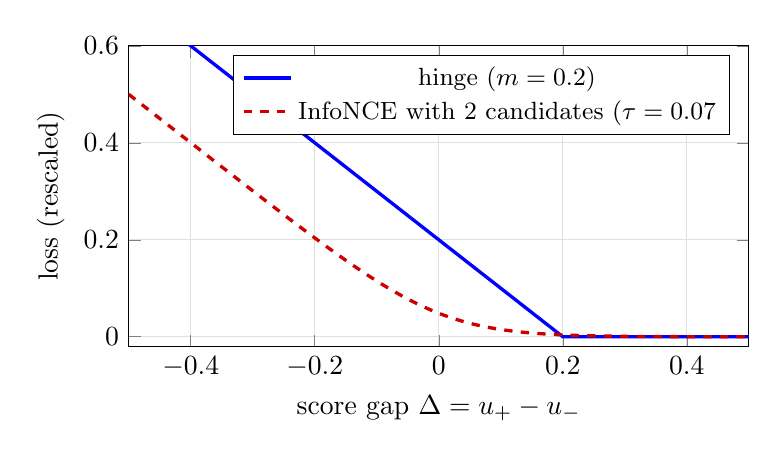
\begin{tikzpicture}
\begin{axis}[width=0.78\linewidth,height=5.4cm,xlabel={score gap $\Delta=u_+-u_-$},ylabel={loss (rescaled)},xmin=-0.5,xmax=0.5,ymin=-0.02,ymax=0.6,grid=both,grid style={gray!25},legend pos=north east,legend style={font=\small}]
\addplot[blue,very thick,domain=-0.5:0.5,samples=201]{max(0,0.2-x)};
\addplot[red!80!black,very thick,dashed,domain=-0.5:0.5,samples=201]{0.07*ln(1+exp(-x/0.07))};
\legend{hinge ($m=0.2$),InfoNCE with 2 candidates ($\tau=0.07$, $\times\tau$)}
\end{axis}
\end{tikzpicture}
\caption{Hinge versus a two-candidate InfoNCE term (new figure; the second is multiplied by $\tau$ so the slopes are comparable). InfoNCE never becomes exactly zero: it keeps pushing already-separated pairs apart.}
\end{figure}
\begin{intuition}
The hinge loss compares the match with \emph{one} negative and a fixed margin. InfoNCE is a cross-entropy over \emph{all} candidates: every other matched pixel acts as a negative and only the exact pixel is rewarded. That gives a much richer learning signal per correspondence, and the low temperature makes the descriptor space sharply peaked.
\end{intuition}

\subsection{Effect of 3D Grounding \slr{41}}
Ablation on the Map-free relocalization benchmark (validation set; estimate the metric pose of a query from a single reference image). All rows take depth from the same monocular depth network.
\begin{center}\small
\begin{tabular}{@{}llccc@{}}\toprule
 & model, matching on & VCRE AUC $\uparrow$ & median error $\downarrow$ & pose AUC $\uparrow$\\\midrule
I & DUSt3R, 3D points & 0.704 & 1.10\,m, 9.4$^\circ$ & 0.344\\
II & MASt3R, 3D points & 0.732 & 0.94\,m, 3.6$^\circ$ & 0.409\\
III & MASt3R, matching loss only, descriptors & 0.744 & 1.10\,m, 10.8$^\circ$ & 0.382\\
IV & MASt3R, descriptors & \textbf{0.752} & \textbf{0.93\,m, 3.0$^\circ$} & \textbf{0.435}\\\bottomrule
\end{tabular}
\end{center}
VCRE AUC: area under the curve of the reprojection error of virtual 3D points under the estimated pose, up to 90\,px. Pose AUC: area under the curve of pose accuracy.
\begin{itemize}
\item Descriptors beat matching on 3D points (II vs.\ IV: $0.732\to0.752$).
\item Without the 3D regression loss, the median rotation error grows from $3.0^\circ$ to $10.8^\circ$ (III vs.\ IV).
\end{itemize}
\begin{intuition}
Descriptors give \emph{precise} matches; the 3D loss gives \emph{geometric sanity}. Row~III shows that a descriptor trained alone has decent reprojection scores but poor rotation -- the matches are locally sharp yet not globally consistent. Training both together gives the best of each.
\end{intuition}

\subsection{Reciprocal Matching \slr{42}}
\begin{Definition}[Reciprocal (mutual nearest-neighbour) matches]
\[ \hat{\mathcal M}=\bigl\{(i,j)\mid j=\NN_2(F^1[i])\ \text{and}\ i=\NN_1(F^2[j])\bigr\},\qquad \NN_2(F^1[i])=\argmin_j\lVert F^2[j]-F^1[i]\rVert, \]
and $\NN_1$ is the same from image~2 to image~1.
\end{Definition}
\begin{Lemma}
$\hat{\mathcal M}$ is a partial one-to-one matching: no pixel of either image appears in more than one pair.
\end{Lemma}
\begin{proof}
If $(i,j),(i,j')\in\hat{\mathcal M}$ then $j=\NN_2(F^1[i])=j'$ (nearest neighbour is a function, ignoring ties); symmetrically for a pixel $j$ appearing with two $i$'s.
\end{proof}
\begin{Example}[1D toy descriptors]
$F^1=(0,\,1,\,5)$ and $F^2=(0.9,\,5.2,\,6)$. Then $\NN_2$ sends $0\to0.9$, $1\to0.9$, $5\to5.2$, while $\NN_1$ sends $0.9\to1$, $5.2\to5$, $6\to5$. Mutual pairs: $(1,0.9)$ and $(5,5.2)$. The pair $(0,0.9)$ is rejected because $0.9$ prefers $1$.
\end{Example}
\begin{itemize}
\item It is the left-right consistency test of Sec.~4.2, applied over the whole image instead of one row.
\item Without rectification there is no epipolar line: every pixel of image~2 is a candidate, so a naive implementation compares all pixel pairs, $O(W^2H^2)$. For a $512\times384$ image this is $\approx3.9\times10^{10}$ pairs (illustrative size).
\end{itemize}
\begin{intuition}
It is the same ``two witnesses must agree'' idea as the left-right test, but without a row to search along. Mutual agreement is a cheap, strong outlier filter; the price is a huge candidate set, which is why MASt3R uses a \emph{fast} matching scheme (the slides name it but do not detail it).
\end{intuition}

\subsection{MASt3R Training Details \slr{43}}
\begin{itemize}
\item \textbf{Data:} 14 datasets (indoor, outdoor, synthetic, real, object-centric), 10 with metric ground truth (Habitat, ARKitScenes, BlendedMVS, MegaDepth, Static Scenes 3D, ScanNet++, CO3D-v2, Waymo, Map-free, WildRGB-D, Virtual KITTI~2, Unreal4K, TartanAir and an internal dataset).
\item \textbf{Amount:} 650k pairs per epoch, equally from all datasets, 35 epochs: $650\text{k}\times35=22.75$ million pairs, batch size 64.
\item \textbf{Images:} 512\,px on the long side, five aspect ratios, random crops and colour jitter.
\item \textbf{Model:} DUSt3R network (ViT-L encoder, ViT-B decoder), initialised from the public DUSt3R checkpoint.
\item \textbf{Optimisation:} AdamW, learning rate $10^{-4}$ with 7 warm-up epochs and cosine decay, weight decay 0.05; 4096 ground-truth correspondences per pair for the matching loss.
\item Hardware and training time: not reported in the paper.
\end{itemize}

\subsection{Results \slr{44}}
\begin{center}\small
\begin{tabular}{@{}lc@{}}\toprule
\multicolumn{2}{@{}l}{\textbf{Map-free relocalization, test set}}\\
method & VCRE AUC $\uparrow$\\\midrule
LoFTR, monocular depth & 0.634\\ DUSt3R & 0.697\\ MASt3R & \textbf{0.933}\\\bottomrule
\end{tabular}\qquad
\begin{tabular}{@{}lccc@{}}\toprule
\multicolumn{4}{@{}l}{\textbf{DTU multi-view stereo, zero-shot (mm)}}\\
method & Acc.\ $\downarrow$ & Comp.\ $\downarrow$ & Overall $\downarrow$\\\midrule
DUSt3R & 2.677 & 0.805 & 1.741\\ MASt3R & \textbf{0.403} & \textbf{0.344} & \textbf{0.374}\\\bottomrule
\end{tabular}
\end{center}
DTU: Acc.\ is the mean distance from the reconstruction to the ground truth (structured light), Comp.\ the reverse, Overall their mean.
\photo{44}{3.4cm}{Grid of object photos/reconstructions from DTU (slide 44, right of the tables).}

\subsection{The Pipeline Revisited \slr{45}}
\begin{center}\small
\renewcommand{\arraystretch}{1.2}
\begin{tabular}{@{}p{2.3cm}p{5.2cm}p{6.6cm}@{}}\toprule
\textbf{Step} & \textbf{Calibrated stereo} & \textbf{MASt3R}\\\midrule
1.\ Calibration & measured offline, required & not needed to match; focal estimated; known intrinsics for the best poses\\
2.\ Rectification & required & not used\\
3.\ Disparity & 1D search along a row & reciprocal nearest neighbours over the whole image\\
4.\ Outliers & left-right consistency test & reciprocity, the same test in 2D\\
5.\ Depth & $z=fb/d$, metric from the measured baseline & pointmap, metric scale from a learned prior\\
6.\ 3D model & fusion of depth maps & pointmaps, or triangulation of the matches\\\bottomrule
\end{tabular}
\end{center}
\textbf{Given up:} a measured metric scale, full resolution (512-pixel windows), low compute, and more than two images per inference.
A calibrated rig still wins for real-time and embedded systems and whenever metric scale must be \emph{measured}.
\begin{intuition}
Each step of the classical recipe has a counterpart, but the machinery moves from ``geometry we measure'' to ``geometry the network has learned''. You gain freedom (arbitrary cameras, wide baselines, forward motion) and lose guarantees (scale, speed, resolution).
\end{intuition}


% =====================================================================
\section*{Summary}\addcontentsline{toc}{section}{Summary}
\subsection*{Comparison of the methods covered}\addcontentsline{toc}{subsection}{Comparison of the methods covered}
\begin{center}\scriptsize
\renewcommand{\arraystretch}{1.25}
\setlength{\tabcolsep}{3pt}
\begin{tabular}{@{}>{\raggedright\arraybackslash}p{2.0cm}>{\raggedright\arraybackslash}p{2.7cm}>{\raggedright\arraybackslash}p{2.5cm}>{\raggedright\arraybackslash}p{2.5cm}>{\raggedright\arraybackslash}p{3.4cm}@{}}\toprule
\textbf{Method} & \textbf{Matching signal} & \textbf{Needs calibration + rectification?} & \textbf{Search / output} & \textbf{Main strength / weakness}\\\midrule
Block matching (SSD/ZNCC) & hand-crafted patch cost, WTA & yes & 1D along row; disparity & simple; noisy, fronto-parallel assumption, border bleeding\\
Siamese CNN (Zbontar--LeCun) & learned cost (MLP) or cosine of learned features & yes & 1D along row; cost volume + WTA/SGM & far less noise; slow if MLP head; ambiguity remains\\
DispNet & correlation layer, end-to-end regression & yes (fixed disparity range) & disparity at several scales & fast, uses synthetic pre-training; rectified input only\\
GC-Net & 3D conv on cost volume, soft argmin & yes (fixed disparity range) & sub-pixel disparity & better accuracy; large memory (3D volume), smoothness bias\\
DUSt3R / MASt3R & pointmaps + 24-d descriptors, reciprocal NN & no (focal estimated) & whole image; pointmap, matches, pose & arbitrary views and wide baselines, scale from a prior; no measured scale, lower resolution, compute heavy\\\bottomrule
\end{tabular}
\end{center}

\begin{figure}[H]\centering
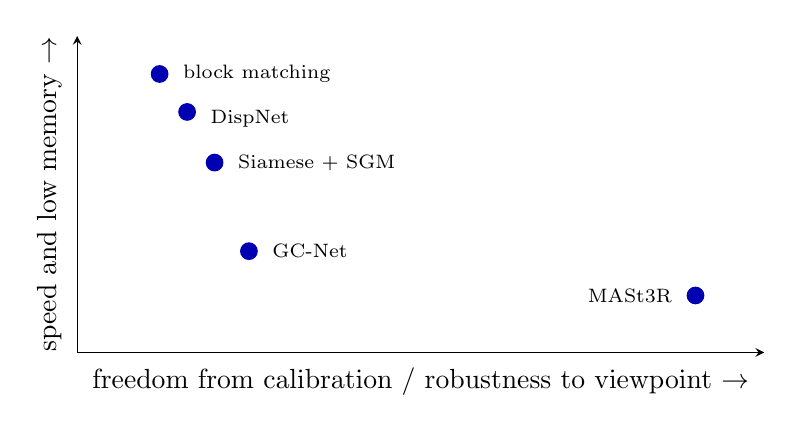
\begin{tikzpicture}
\begin{axis}[width=0.85\linewidth,height=5.6cm,xlabel={freedom from calibration / robustness to viewpoint $\rightarrow$},ylabel={speed and low memory $\rightarrow$},
 xmin=0,xmax=10,ymin=0,ymax=10,xtick=\empty,ytick=\empty,grid=both,grid style={gray!20},axis lines=left,
 nodes near coords style={font=\scriptsize}]
\addplot[only marks,mark=*,mark size=3pt,blue!70!black] coordinates {(1.2,8.8)(2.0,6.0)(1.6,7.6)(2.5,3.2)(9.0,1.8)};
\node[anchor=west,font=\scriptsize] at (axis cs:1.4,8.8) {block matching};
\node[anchor=west,font=\scriptsize] at (axis cs:2.2,6.0) {Siamese + SGM};
\node[anchor=west,font=\scriptsize] at (axis cs:1.8,7.4) {DispNet};
\node[anchor=west,font=\scriptsize] at (axis cs:2.7,3.2) {GC-Net};
\node[anchor=east,font=\scriptsize] at (axis cs:8.8,1.8) {MASt3R};
\end{axis}
\end{tikzpicture}
\caption{Qualitative placement of the methods on two axes, drawn from the discussion on the slides (calibration/rectification dependence, memory and compute); positions are \emph{not} measured values.}
\end{figure}

\subsection*{Key take-aways}\addcontentsline{toc}{subsection}{Key take-aways}
\begin{itemize}
\item \textbf{Geometry buys you a 1D search.} With calibration and rectification, matching is along a scanline (a $480\times$ smaller search for VGA) and depth follows from $z=fb/d$.
\item \textbf{Stereo error is quadratic in depth:} $\delta z\approx z^2\delta d/(fb)$. A wider baseline helps the arithmetic but makes matching harder.
\item \textbf{Block matching fails where local similarity fails} (occlusions, slanted surfaces, repetitions, textureless areas); window size trades noise against border bleeding, and the left-right consistency test removes many outliers.
\item \textbf{Learning replaced the hand-made parts in two steps:} learned matching costs (Siamese nets, hinge loss on triplets), then end-to-end networks (DispNet, GC-Net with cost volumes and soft argmin) -- still tied to rectified input and a fixed disparity range.
\item \textbf{Matching in 3D drops calibration and rectification from the matching step} (DUSt3R/MASt3R: pointmaps, descriptors, reciprocal matching) at the price of measured metric scale, resolution, compute and the number of views; calibrated rigs still win for real-time and embedded, metrically accurate use.
\end{itemize}

\end{document}